\documentclass[a5paper,pagesize]{scrbook}

\usepackage[T1]{fontenc}
\usepackage[utf8]{inputenc}

\usepackage{amssymb}
\usepackage{authblk}
\usepackage[ngerman]{babel}
\usepackage[natbib,notes,backend=bibtex]{biblatex-chicago}
   \bibliography{references}
\usepackage{booktabs}
\usepackage{CormorantGaramond}
\usepackage[german=guillemets]{csquotes}
\usepackage{enumitem}
   \setlist{noitemsep}
\usepackage{float}
\usepackage{graphicx}
   \graphicspath{{figures/}}
\usepackage[hidelinks]{hyperref}
   \urlstyle{same}
\usepackage{longtable}
\usepackage{microtype}
\usepackage{siunitx}
\usepackage{tabto}
\usepackage{tikz}
\usepackage[normalem]{ulem}
\usepackage{url}

\addtokomafont{disposition}{\rmfamily}

\setlength{\fboxsep}{0pt}
\setlength{\fboxrule}{1pt}

\deffootnote{1.5em}{1em}{\makebox[1.5em][l]{\thefootnotemark}}
   \setlength{\skip\footins}{1.5em}
   \setlength{\footnotesep}{1em}

\title{Gothic}
\subtitle{}

\author{Alexander Max Bauer}

\date{}


%%%%%%%%%%%
% TITELEI %
%%%%%%%%%%%
\begin{document}
\maketitle


%%%%%%%%%%%%%%%%%%%%%%
% INHALTSVERZEICHNIS %
%%%%%%%%%%%%%%%%%%%%%%
\frontmatter
\tableofcontents


%%%%%%%%%%%
% VORWORT %
%%%%%%%%%%%
\mainmatter
\chapter{Ein Wort vorab}\label{ch:vorwort}


%%%%%%%%%%%
% QUELLEN %
%%%%%%%%%%%
\chapter{Ein Wort zu den Quellen}\label{ch:quellen}
Darüber, ob Videospiele als Kunst gelten und als legitimer Gegenstand wissenschaftlicher Untersuchung oder philosophischer Reflexion betrachtet werden können, scheint glücklicherweise immer weniger Dissens zu herrschen.\footnote{In diesem Sinne ernstgenommen werden sie etwa -- um aus der Vielzahl vorhandener Publikationen nur drei ausgewählte Beispiele zu nennen -- von \autocite{feige_computerspiele_2015}, \autocite{zimmermann_gameskultur_2020} sowie \autocite{beil_game_2018}.}
Wie Literatur, Gemälde oder Filme werden sie damit zunehmend auch als etwas betrachtet, das es zu bewahren und zugänglich zu machen gilt.
In diesem Bewusstsein sind inzwischen sowohl in Deutschland wie auch international zahlreiche Sammlungen -- einige in privater Hand, andere in öffentlicher Trägerschaft -- entstanden, deren Bestand an Videospielen bis in die Zehntausende reicht.
Sebastian Möring resümiert:

\begin{quote}
   Die nach eigener Auskunft größte private Computerspielsammlung ist mit 10.000 Spielen das Haus der Computerspiele.
   Sie wurde vom Leipziger Journalisten René Meyer initiiert.
   Die Sammlung des Computerspielemuseums in Berlin mit bis zu 30.000 Exemplaren geht auf die Initiative des Fördervereins für Jugend und Sozialarbeit (fjs e.\,V.) zurück.
   Sie ist damit die größte institutionalisierte Sammlung in Deutschland.
   Über die größte Sammlung an einer deutschen Hochschule verfügt das DIGAREC -- Zentrum für Computerspielforschung der Universität Potsdam mit etwa 10.000 Spieletiteln.
   Auf internationaler Ebene sammeln etablierte Kulturinstitutionen wie das Museum of Modern Art (MoMA) und die Library of Congress in den USA oder die Königliche Bibliothek in Dänemark.
   Hierzulande erweitert das renommierte Deutsche Literaturarchiv Marbach seinen Sammlungsauftrag und schließt Computerspiele darin ein.\autocite[S.~120]{moering_kulturarchive_2020}
\end{quote}

Vielleicht lässt sich schon hieran -- mit aller gebotenen Vorsicht -- ein Trend darin erkennen, wie mit Videospielen und dem sie umgebenden Kosmos als bewahrenswerte Kulturgegenstände umgegangen wird.
\enquote{Am Anfang}, schreibt Möring, \enquote{steht bei den meisten Sammlungen die Frage nach den Objekten, welche gesammelt werden sollen.}\autocite[S.~121]{moering_kulturarchive_2020}
Das sind in erster Linie die Spiele selbst, also die entsprechende Software, eng damit verbunden aber auch die dazugehörigen Speichermedien und in einigen Fällen die benötigte historische Hardware, um die Spiele spielen zu können, wenn man nicht auf Emulatoren ausweichen möchte.
Aus dem sie umgebenden Kosmos werden daneben aber auch \enquote{Zeitschriften und Bücher zu Computerspielen gesammelt sowie Actionfiguren, Comics, Filme}\autocite[S.~121]{moering_kulturarchive_2020} und dergleichen mehr.
Der Fokus scheint, wenig verwunderlich, auf offiziell veröffentlichtem Material zu liegen.
Nur vergleichsweise selten widmet man sich den Vorstufen dieses Materials, den groben Ideenskizzen, den frühen Entwürfen und Designdokumenten, den Alpha- und Betaversionen der Spiele, den internen Entwicklungswerkzeugen und so weiter.
All das ist in der Regel -- anders als das fertige Spiel -- nur selten dafür bestimmt, in die Öffentlichkeit entlassen zu werden, sieht man von dem ein oder anderen Making-of-Buch oder Bildband mit Konzeptzeichnungen ab.
Entsprechend konstatiert Nico Nolden:
\enquote{Ungenutzt schlummern Artworks (Konzeptzeichnungen und ähnliches), Prototypen und Designdokumente in Firmenarchiven, die sich auf‌lösen, sobald die Unternehmen eingehen.}\autocite[S.~44]{nolden_geschichte_2020}

Nur sporadisch finden einzelne Dokumente oder Entwicklungsversionen von Spielen ihren Weg in die Öffentlichkeit, wobei oft nur noch mit Mühe nachzuvollziehen ist, wie dieser Weg aussah.
Durch die Weiten des Netzes geistern unter anderem -- um nur ein paar Beispiele zu nennen -- Designdokumente von \textit{Diablo} (1996), \textit{Doom} (1993), dem nie erschienenen \textit{Fallout: Brotherhood of Steel 2}, \textit{Grim Fandango} (1998), \textit{Planescape: Torment} (1999), \textit{Silent Hill} (1999) oder \textit{Tron} (1982).\footnote{Diese Beispiele hat Mikael Segedi gesammelt und zugänglich gemacht; \autocite[vgl.][]{segedi_famous_2015}.}

Manchmal sammeln Liebhaber*innen solche Dokumente online, wie beispielsweise im Fall von \textit{Tomb Raider} oder \textit{Gothic}.\autocite[Vgl.][]{core_design_tomb_raider,gothic_archive_2024}
In einigen Fällen wird eine solche Veröffentlichung aber auch von Entwickler*innen oder Publishern selbst forciert.
Al Lowe beispielsweise hat auf seiner Homepage unter anderem Dokumente zu \textit{Leisure Suit Larry 5: Passionate Patti Does a Little Undercover Work} (1991), \textit{Leisure Suit Larry 6: Shape Up or Slip Out!} (1993) und \textit{Leisure Suit Larry 7: Love for Sail!} (1996) zugänglich gemacht.\autocite[Vgl.][]{lowe_designs_2025}
Auch Aric Wilmunder hatte auf seiner -- inzwischen nicht mehr erreichbaren -- Homepage eine ganze Reihe von Designdokumenten veröffentlicht, die sich über lange Jahre in seinem Besitz befanden.
Unter der Überschrift \enquote{A Peek Into My Games Industry Archive} hatte er die eingescannte Sammlung mit den Worten eingeleitet:

\begin{quote}
   Monkey Island, Day of the Tentacle, Maniac Mansion, The Dig, Indy Iron Phoenix, the list goes on.
   I worked on all of these and had a suspicion that someday there would be interest in how these games were made.
   Years ago I visited the LucasArts facility in the San Francisco Presidio and brought along two grocery bags of design documents.
   I asked if they had an archivist and I was told that since I had kept these safe for over two decades, it was best if I just kept them together.
   I have met with the archivist at Stanford and these documents will either end up there or at a museum dedicated to preserving game design.\autocite{wilmunder_peek}
\end{quote}

Darunter fanden sich Dokumente unter anderem zu \textit{The Secret of Monkey Island} (1990), \textit{The Curse of Monkey Island} (1997), \textit{Indiana Jones and the Last Crusade} (1989), dem nie erschienenen \textit{Indiana Jones and the Iron Phoenix}, \textit{Maniac Mansion} (1987), \textit{Sam \& Max Hit the Road} (1993), \textit{Star Wars: Rebel Assault} (1993) oder \textit{The Dig} (1995).\footnote{Zu \textit{Maniac Mansion} und \textit{The Curse of Monkey Island} lohnt sich auch ein Blick auf Ron Gilberts Website; \autocite[vgl. etwa][]{gilbert_maniac_mansion_2014}.}
Andere -- inzwischen ebenso nur noch über die \textit{Wayback Machine} des \textit{Internet Archive} erreichbare -- Beispiele sind Richard Hill-Whittall, der eine Reihe von Dokumenten zu Wii- und PSVita-Spielen auf seiner Homepage veröffentlicht hatte,\autocite[Vgl.][]{hill_whittall_gdd_2017} Mike Dailly, der das Designdokument von \textit{Grand Theft Auto} (1997) auf \textit{Flickr} hochgeladen hatte,\footnote{\autocite[Vgl.][]{dailly_race_n_chase_2011}; zum zweiten Teil siehe außerdem \autocite{internet_archive_gta_2}.} Deep Silver Volition, die Dokumente des nie erschienenen \textit{Saints Row: Undercover} veröffentlicht hatten\footnote{\autocite[Vgl.][]{volition_thursday_2016}. \enquote{Nie erschienen} trifft es dabei nicht ganz: Im gleichen Zuge hat Volition damals auch eine spielbare Entwicklungsversion zugänglich gemacht; \autocite[vgl.][]{frank_canceled_2016}.} oder Giant Sparrow, die einen internen Trailer und Dokumente von \textit{What Remains of Edith Finch} (2017) auf ihrem Blog gepostet hatten.\autocite[Vgl.][]{giant_sparrow_edith_2018}

Daneben gibt es auch einige Entwickler, die -- wahrscheinlich nicht ohne ein gewisses videospielhistorisches Selbstverständnis und -bewusstsein -- eigene Editionen ihrer Notizen herausgebracht haben, etwa Jordan Mechner zu seinen Spielen \textit{Karateka} (1984) und \textit{Prince of Persia} (1989) mit \textit{The Making of Karateka} und \textit{The Making of Prince of Persia} oder Zach Barth mit \textit{Zach-Like}.\autocite[Vgl.][]{mechner_karateka_2012,mechner_prince_2020,barth_zach_like_2019}
In jüngster Zeit hat außerdem die von Frank Cifaldi gegründete \textit{Video Game History Foundation} die Tore ihrs digitalen Archivs geöffnet.
Die mehr als 30.000 Archivalien umfassen neben Videospielmagazinen, Artworks, Pressemappen und anderem Werbematerial auch \enquote{[n]ever-before-seen game development materials.}\autocite{salvador_library_2025}

Dass diese Fälle eher Ausnahmen zu bleiben und der Fokus von Sammlungen in erster Linie auf offiziell veröffentlichtem Material zu liegen scheint, ist wenig verwunderlich.
Wahrscheinlich halten die meisten Kunstschaffenden die Vorstufen ihrer Werke zu Lebzeiten zurück; viele Sammlungen speisen sich vermutlich vorrangig aus dem Nachlass.
Daneben sind immer -- sowohl zu Lebzeiten von Künstler*innen wie auch danach -- rechtliche Fragen zu klären.
Außerdem sind viele Spiele nicht das Werk einer einzelnen Person, sondern ganzer Gruppen.
Hier ist unter Umständen also zusätzlich ein komplexes Netz geistigen Eigentums zu beachten.
Zudem entstehen Videospiele überwiegend im Kontext von Unternehmen, also von marktwirtschaftlich agierenden Gruppen, die sich wahrscheinlich oft nicht in die eigenen Karten der Spieleproduktion blicken lassen möchten.

Trotz solcher Schwierigkeiten plädiere ich dafür, dass diese oft unveröffentlichten Dokumente als wichtige Quellen für die Videospielforschung angesehen werden.
Gleiches gilt meiner Meinung nach übrigens auch -- aber das soll an dieser Stelle nur eine Randbemerkung bleiben -- für Kommunikation beispielsweise über E-Mail.\footnote{An vielen Stellen profitiert die Forschung von dem erhalten gebliebenen Schriftverkehr vergangener Generationen.
Dass ein Großteil dieses Schriftverkehrs heute elektronisch vonstattengeht und das Risiko birgt, für künftige Generationen unzugänglich zu werden, haben Errol Friedberg und Kollegen bereits Anfang des Jahrtausends in einer Zuschrift an \textit{Nature} angemaht; \autocite[vgl.][]{friedberg_e_mail_2003}.}
Für mich stellen solche Dokumente ein Analogon dar zu Vorstufen, Vorskizzen, Notizen, Briefen und all den anderen Hintergrunddokumenten, die wir heranziehen, wenn wir uns Schriften oder Kunstwerken eingehender widmen.
Denkt man diesen Gedanken weiter, muss man sich fragen, wie solche Dokumente aus dem Kosmos der Videospiele archiviert, zugänglich gemacht und aufbereitet werden können.
Hier liegt ein Brückenschlag zur Editionswissenschaft nahe.
Immerhin: Wenn Bodo Plachta das Folgende in seiner Einführung in die Editionswissenschaft schreibt, scheint es mir vor diesem Hintergrund nicht so abwegig, das erste Wort -- \enquote{Texte} -- durch \enquote{Videospiele} zu ersetzen:

\begin{quote}
   Texte sind historische Dokumente.
   Ihre Entstehung und die aus ihr resultierenden Ergebnisse müssen als ein historischer Prozeß beschrieben und fixiert werden.
   Diesen Entstehungsprozeß in seiner Komplexität aus historischen, biographischen oder poetologischen Komponenten möglichst umfassend zu dokumentieren und zu erläutern, ist ein wichtiges Ziel der historisch-kritischen Ausgabe.
   Dazu ist es notwenig, nicht nur sämtliche Materialien eines zu edierenden Werkes oder Textes zu sichten, sondern die Arbeitsstadien aus diesem Material zu ermitteln, diese zur Entstehung in Beziehung zu setzen und den zu rekonstruierenden Entstehungsprozeß in seiner ganzen Komplexität bis zu einer eventuellen Publikation zu verfolgen.\autocite[S.~13\,f.]{plachta_editionswissenschaft_1997}
\end{quote}

Ich möchte unterstreichen, dass Videospiele es, wenn man sie als Kulturgüter begreift, verdient haben, nicht nur in ihrem Ergebnis, sondern auch in ihrer Entstehung ernst genommen zu werden.
Und das heißt -- nicht in allen, aber doch in einigen Fällen --, ebenso ernst genommen zu werden wie ein Text von Kafka oder Shelley, ein Gemälde von Dürer, eine Grafik von Kollwitz oder eine Komposition von Pejačević.
In diesem Band möchte ich versuchen, \textit{Gothic} in diesem Sinne ernst zu nehmen.
Er soll keine historisch-kritische Bearbeitung bieten; generell verstehe ich das Vorliegende nicht als eine wissenschaftliche Arbeit im engeren Sinne.
Aber es mag sich durchaus lohnen, einmal probeweise einen genaueren Blick auf solche Hintergrunddokumente zu werfen und sich zu fragen, was sie uns über die Entstehungsgeschichte eines Spiels erzählen können.


%%%%%%%%%%%%%%%%%%%%%%%%%%%%%
% QUELLEN – ARCHIVDOKUMENTE %
%%%%%%%%%%%%%%%%%%%%%%%%%%%%%
\section{Archivdokumente}\label{ch:quellen_archivdokumente}
Wird ein Archivdokument das erste Mal eingehender behandelt, stelle ich es mit einer äußerst knappen Handschriften- beziehungsweise Dokumentenbeschreibung vor.

Bei Zitaten aus solchen Dokumenten erfolgt eine buchstabengetreue Wiedergabe.
Auch die Interpunktion wird unverändert übernommen.
Abkürzungen werden nicht aufgelöst.
Fehler in Orthographie oder Interpunktion bleiben ebenfalls erhalten.
Statt sie zu korrigieren, weise ich an den entsprechenden Stellen in eckigen Klammern mit dem lateinischen \textit{sic} (\enquote{so}, von \textit{sic erat scriptum}, \enquote{so wurde es geschrieben}) darauf hin, dass die jeweilige Stelle in dieser Form aus der Vorlage stammt.
Andere Kommentare, Ergänzungen, Anpassungen und Auslassungen von mir werden ebenfalls durch eckige Klammern kenntlich gemacht.
Finden sich in der Vorlage Hervorhebungen oder Korrekturen (beispielsweise fette oder kursive Schriften, Unterstreichungen, Sperrungen oder Durchstreichungen), werden diese übernommen.
Damit hoffe ich, eine \enquote{Einebnung typographischer Besonderheiten} zu vermeiden, die sonst \enquote{auch mit einer Sinnverlagerung einhergehen kann}.\autocite[S.~21]{plachta_editionswissenschaft_1997}

Zeilen- oder Seitenwechsel werden dagegen nicht ausgewiesen.
Worttrennungen am Zeilenende werden entsprechend aufgelöst und Trennzeichen getilgt.
Auch Textfarben werden -- außer bei Erwähnung in Handschriften- oder Dokumentenbeschreibung -- nicht ausgewiesen.

Ich versuche, das Quellenmaterial möglichst für sich sprechen zu lassen, weswegen ich zahlreich daraus zitiere.
Um den Fußnotenapparat nichtsdestotrotz möglichst schlank halten zu können, weise ich nicht jedes einzelne Zitat mit genauer Fundstelle aus, solange deutlich ist, aus welchem Archivdokument es stammt.


%%%%%%%%%%%%%%%%%%%%%%%%
% QUELLEN – INTERVIEWS %
%%%%%%%%%%%%%%%%%%%%%%%%
\section{Interviews}\label{ch:quellen_interviews}


%%%%%%%%%%%%%%
% WILLKOMMEN %
%%%%%%%%%%%%%%
\chapter{Willkommen im Lager}\label{ch:willkommen}
Gothic beginnt mit einem kurzen Video, das die Prämisse des Spiels in wenigen Minuten vorstellt.
Der Bildschirm ist noch schwarz, als die markante Stimme des Sprechers Bodo Henkel anhebt:
\enquote{Das Königreich Myrtana, wiedervereint durch die Hand König Rhobars II.}
Eine Aufblende führt uns in einen kargen Thronsaal.
Die Kamera bewegt sich, einem roten, von Säulen gesäumten Läufer folgend, auf den König zu, der mit geneigtem Haupt, sich auf eine Lanze stützend, an der Stirnwand des Saals auf seinem schmucklosen Thron sitzt.
Er trägt eine reich verzierte Brustplatte, um seine Schultern liegt ein Fell, die Hände stecken in schweren Panzerhandschuhen.
Durch gothische Fenster fällt von rechts Licht in den steinernen Raum.
\enquote{In den langen Jahren seiner Herrschaft war es ihm gelungen, alle Widersacher des Reiches zu bezwingen}, erfahren wir.

Ein weite Ebene; im Hintergrund ein verfallenes Haus und ein einsamer kahler Baum.
\enquote{Bis auf einen}, fügt der Sprecher an.
Der Fuß eines Orks wirbelt Staub vom Boden auf.
Hinter ihm stürmt eine ganze Armee von seinesgleichen mit gezogenen Waffen vorwärts.
Eine Handvoll menschlicher Bogenschützen setzt zum Schuss an.
Von irgendwoher ertönt das Kommando: \enquote{Feuer!}
Einige Orks fallen den Pfeilen zum Opfer, die meisten aber stürmen unbeirrt weiter.
Ihre großen, grob gearbeiteten Waffen machen mit den Bogenschützen kurzen Prozess.

Eine unterirdische, von Fackelschein erleuchtete Miene.
Arbeiter schwingen ihre Spitzhacken, hinter ihnen stehen Wächter, ihre Arme in die Seiten gestemmt, auf dem Boden Haufen blauen Erzes.
Ein Arbeiter trägt zwei schwere Säcke mit einem Tragejoch auf seine Schultern.
\enquote{Der Krieg mit den Orks forderte seinen Tribut}, fährt der Sprecher fort, \enquote{und die Gefangenen des Reiches sollten ihn bezahlen.
Der König brauchte Schwerter für seine Armeen -- und jeder, der sich eines auch noch so geringen Verbrechens schuldig gemacht hatte, wurde zur Arbeit in den Erzminen von Khorinis gezwungen.}
Im nächtlichen Fackelschein bewegt sich eine Reihe aneinandergeketteter Häftlinge, die Hände auf dem Rücken gefesselt, auf eine Burg zu.
Wächter in imposanten Rüstungen stehen an der Seite des Trosses.

Dunkle Bäume heben sich vor einem abendlichen Himmel ab.
\enquote{Um jede Flucht unmöglich zu machen, sandte der König die mächtigsten Magier des Reiches aus, eine magische Barriere um das gesamte Tal zu errichten.}
Eine Figur materialisiert sich in einer blau leuchtenden Wolke aus dem Nichts.
Sie trägt eine blaue Robe, das Gesicht unter einer Kapuze verborgen.
Mit beiden Händen hält sie einen Stab, den sie vor sich in den Boden rammt.
Blaue Blitze zucken um ihren Körper und springen auf einen blauen Kristall über, der an der Spitze des Stabes in einer Fassung aus vier Sicheln gehalten wird.
\enquote{Ich war einer der Magier}, erfahren wir.
Die Sicheln geben den Kristall frei, der sich in einen Ball aus Energie zu verwandeln scheint und in Richtung der Burg fliegt, deren nächtliche Silhouette wir schon gesehen haben.
Aus anderen Richtungen fliegen zwei weitere blaue Kugeln und alle drei treffen sich hoch oben, über der Burg, in einem gewaltigen Funkenregen.
Eine blau schimmernde Kuppel beginnt sich vom Ort ihrer Kollision her auszubreiten.
\enquote{Aber etwas störte das gebrechliche Gefüge der Magie.}
Die Kuppel wächst im rasanten Tempo immer weiter und umschließt bald auch den Magier in der blauen Robe.
\enquote{Wir waren nun selbst Gefangene der Barriere.}

Im Innenhof der Burg stehen zwei Wachen, die verwundert in den Himmel, auf die gerade entstandene blau schimmernde Kuppel, blicken.
Eine der beiden weist mit der Hand nach oben, als sich von hinten vorsichtig ein Arbeiter nähert und ihr eine Spitzhacke in den Rücken rammt.
\enquote{Mehr als eine Sekunde der Unachtsamkeit brauchten die Gefangenen nicht.}
Der Arbeiter zieht seine Spitzhacke aus der bäuchlings auf dem Boden liegenden Wache, ein anderer schneidet einer weiteren derweil von hinten mit dem Messer die Kehle durch.
\enquote{Khorinis war nun in den Händen der Gefangenen.}

\enquote{Der König hatte keine Wahl.}
Rhobar II. erhebt sich von seinem Thron, um einem Boten eine Schriftrolle zu übergeben.
Der wirft sie durch die Barrier, wo sie vor den Füßen eines Häftlings landet.
\enquote{Er musste verhandeln, er brauchte das Erz.}
Kisten, Fässer, Säcke, eine leicht bekleidete Frau, die Hände auf den Rücken gebunden, werden von einer erhöht liegenden Plattform aus mit einem hölzernen, von einer eisernen Kette gezogenen Aufzug in das Innere der Barriere befördert.
Der Frau entfährt ein Schmerzenslaut, als sie den Rand der magischen Kuppel passiert.
\enquote{Monat für Monat lieferte der König den Gefangenen alles, was sie verlangten.
Monat für Monat brachten sie dafür das Erz an den Rand der Barriere.
In all den Jahren wurden viele Versuche unternommen, die magische Barriere zu öffnen, aber keiner hatte Erfolg.}

Obwohl im Inneren der Kuppel nun die Häftlinge das Sagen haben, hat das Mienental seine Funktion als Gefängnis nicht verloren.
Flankiert von zwei Wächtern wird ein neuer Gefangener an den Rand einer Klippe geführt, hinter deren Abgrund die magische Barriere schimmert.
Seine beiden Bewacher halten ihm die Arme auf dem Rücken, während vor ihm ein Richter in gelber Robe und mit einem hohen, farblich passenden Hut, sein Urteil zu verlesen beginnt:
\enquote{Im Namen König Rhobars II., Träger des Zepters von Varant, Vereiniger der vier Reiche am Myrth$\ldots$}
Weiter kommt er nicht, denn eine Figur in rot-schwarzer Robe tritt hinzu und unterbricht ihn mit einem gebieterischen \enquote{Halt}, ehe sie sich an den Häftling wendet und fortfährt:
\enquote{Gefangener, ich habe dir ein Angebot zu machen:
Dieser Brief \textit{muss} den Führer der Feuermagier erreichen.}
Der Angesprochene aber gibt sich unbeeindruckt:
\enquote{Du verschwendest deine Zeit}, gibt er zurück.
\enquote{Deine Belohnung}, erwidert der Hinzugekommene in verlockendem Ton, \enquote{könntest du selbst wählen.
Man wird dir alles geben, was du verlangst.}
Das war hinreichend überzeugend:
\enquote{Gut}, antwortet der Gefangene mit einem schelmischen Lächeln im Gesicht, {ich werde deinen Brief nehmen.}
Die beiden Bewacher geben seine Arme frei, damit er das Schriftstück an sich nehmen kann, als er forfährt:
\enquote{Unter \textit{einer} Bedingung}, er zeigt auf den Richter, \enquote{Erspart mir den Rest von seinem Gefasel!}
Der Vertreter des Gesetzes möchte sich empören:
\enquote{Du wag$\ldots$}, hebt er an, wird aber erneut von dem Magier unterbrochen:
\enquote{Schweig.}
Es besteht wenig Zweifel daran, wer von beiden in diesem Moment die höhere Autorität genießt.
Und so ist es der Magier, der fortfährt:
\enquote{Gut, hinein mit ihm.}
Seine beiden Bewacher stoßen den Häftling über den Rand der Klippe, wo er durch die magische Barriere fällt und in einem See landet.
Als er sich an das Ufer schleppt, wird er von drei rot gewandeten Gestalten empfangen.
Einer von ihnen zieht ihn mit den Worten \enquote{Willkommen im Lager} zu sich herauf -- und verpasst ihm einen Faustschlag mitten ins Gesicht.
Für einen Augenblick ist alles Schwarz.
Bis man von irgendwoher hört:
\enquote{Das reicht, lasst ihn in Ruhe.
Macht, dass ihr wegkommt.}
Als er die Augen wieder aufschlägt, steht eine andere, im gleichen dunklen Rot gekleidete Person vor dem Häftling.
\enquote{Steh' auf}, sagt sie.

Damit endet das kurze Video, das den Beginn von Gothic markiert.
Für einen Augenblick schaut man, nun in der Spielgrafik, von hinten auf den Häftling, der in der Mitte des Bildschirms steht.
Spätestens jetzt wird klar:
Dieser Häftling, das ist die Spielfigur.
Das sind wir.
Vor uns steht die rotgekleidete Person, die einen Augenblick zuvor die drei anderen vertrieben hat.
Sie trägt breit auslaufende schwarze Schulterplatten und eine bauschige, aus roten und schwarzen Quadraten zusammengeflickte Hose, die in seinen Stiefeln zu stecken scheint.
Seine Hände werden von schweren Handschuhen geschützt; darüber sind die Arme nackt.
An seinem Gürtel baumelt ein Schwert und über die Schulter hat er einen Bogen geworfen, der so groß ist, wie er selbst.
\enquote{Ich bin Diego}, stellt er sich vor.
\enquote{Ich bin$\ldots$}, setzen wir an, werden von ihm aber augenblicklich unterbrochen:
\enquote{Mich interessiert nicht, wer du bist.}
Das ganz Spiel hindurch werden wir ohne Namen bleiben, weswegen die Spielfigur in der Community den passenden Beinamen des \textit{Namenlosen Helden} erhalten hat.
Aber noch sind wir kein Held, sondern nur ein weiterer Gefangener.
\enquote{Du bist neu hier}, fährt Diego fort, \enquote{Ich kümmere mich um die Neuen.
Belassen wir es vorerst dabei.
Wenn du vorhast, länger zu leben, solltest du dich ein bisschen mit mir unterhalten.
Ich werde dich allerdings nicht daran hindern, in dein Verderben zu rennen.
Also, wie sieht's aus?}

Diego meint, was er sagt.
Nichts hindert uns daran, direkt weiter unserer Wege zu ziehen.
In diesem Fall verabschiedet sich Diego mit einem trockenen \enquote{Wie du willst.
War nett, dich gekannt zu haben.}
Wenn wir Gothic allerdings zum ersten Mal und ohne Vorwissen spielen, entgeht uns dadurch auch ein guter Teil der Exposition -- und der ein oder andere Tipp, der tatsächlich dafür sorgen könnte, dass wir etwas länger am Leben bleiben.
Deswegen wählen wir aus den zur Verfügung stehenden Optionen zuallererst die oberste aus, woraufhin unser namenloser Held, markant vertont von Christian Wewerka, entgegnet:
\enquote{Okay, was muss ich über diesen Ort wissen?}

Wir erfahren von Diego, dass das Kuppelgefängnis als die \enquote{Kolonie} bezeichnet wird und dass sich in ihm drei Lager gebildet haben.
Das älteste davon, dem auch Diego angehört, wird schlicht das \enquote{Alte Lager} genannt.
\enquote{Es ist das größte und mächtigste der drei Lager}, erläutert er.
\enquote{Gomez und seine Jungs kontrollieren das Lager und damit den ganzen Erzaustausch.
Einmal im Monat schickt der König uns alles, was wir fordern.
Wir haben den alten Sack in der Hand, verstehst du?
Er ist auf das Erz angewiesen.
Er schickt uns Wein, Brot, Fleisch, Waffen, einfach alles.
Du kannst auch deinen Teil davon bekommen.
Alles, was du tun musst, ist dich Gomez' Leuten anzuschließen.}
Dieser Machtstellung halber werden Gomez und seine Jungs auch als Erzbarone bezeichnet.
\enquote{Die beiden anderen Lager}, erklärt uns Diego, \enquote{haben sich abgespalten, um ihren schwachsinnigen Ausbruchsplänen nachzugehen.
Es gibt das neue Lager im Westen der Kolonie.
Die Magier dort meinen, wenn sie genug Erz zusammengekratzt haben, können sie die Barriere einfach sprengen.
Dann gibt's im Osten die Sektenspinner.
Sie haben ihr Lager im Sumpf und beten zu ihrem Götzen, er möge ihnen die Freiheit schenken.
Bis jetzt hat er sich noch nicht gemeldet.}

Wenn wir möchten, können wir Diego von dem Brief erzählen, den uns der Magier gegeben hat, ehe wir von der Klippe gestoßen wurden.
\enquote{Du kannst von Glück sagen, dass ich mich bei den Magiern nicht mehr blicken lassen kann}, erwidert Diego, \enquote{Jeder andere wird dir mit Freude für diesen Brief die Kehle durchschneiden.
Die Magier belohnen ihre Boten immer sehr gut, und die meisten hier haben gar nichts, verstehst du?
Wenn ich du wäre, würde ich die Schnauze halten, bis ich einen der Magier treffe.
Obwohl das in deiner Lage nicht allzu wahrscheinlich ist.}
Die Magier, erfahren wir, residieren in der Burg des Alten Lagers.
Zutritt zur Burg haben allerdings nur Gomez und seine Leute.

Da trifft es sich gut, dass es nicht nur reine Nächstenliebe war, aus der heraus Diego uns geholfen hat:
\enquote{Bullit und seine Jungs hätten dich vielleicht kaltgemacht}, sagt er.
\enquote{Und das konnte ich nicht mit ansehen.
Schließlich bin ich den ganzen weiten Weg gekommen, um dir einen Vorschlag zu machen.}
\enquote{Einen Vorschlag?}, haken wir nach.
\enquote{Ja}, sagt Diego, \enquote{Deine Begegnung mit Bullit und seinen Jungs hat dir hoffentlich gezeigt, dass du Schutz brauchst.
Jeder, der hier ankommt, wird vor eine Wahl gestellt.
Es gibt drei Lager in der Kolonie, und einem davon wirst du dich anschließen müssen.
Ich bin hier, um Neuen wie dir klarzumachen, dass sie bei uns im alten Lager am besten aufgehoben sind.}
Sollten wir uns dem alten Lager anschließen wollen, sollen wir am Eingang der Burg nach einem Mann namens Thorus Ausschau halten und ihm sagen, dass Diego uns schickt.
Auch eine Wegbeschreibung gibt er uns an die Hand:
\enquote{Du musst nur dem Weg hier folgen.
Das Alte Lager ist der nächste halbwegs sichere Ort von hier aus gesehen.}
Wir erfahren außerdem, dass Bullit, dem wir das blaue Auge zu verdanken haben, ebenfalls im Alten Lager zu finden ist.
\enquote{Aber wenn du vorhast, dich mit ihm anzulegen, sei vorsichtig}, warnt uns Diego, \enquote{Er ist ein erfahrener Kämpfer.}
Nicht nur Bullit ist eine warnende Erwähnung wert.
\enquote{Es treiben sich jede Menge wilder Bestien zwischen den Lagern herum}, erzählt Diego, \enquote{Ohne Waffe zu gehen ist Wahnsinn.}
Auf dem Weg zum Alten Lager sollen wir uns ein bisschen umschauen, rät er.
Irgendeine alte, noch brauchbare Waffe werden wir dort schon finden.

Auch auf die Barriere können wir Diego ansprechen.
\enquote{Was passiert, wenn ich hier einfach wieder rausspaziere?}, fragen wir ihn.
\enquote{Der Letzte, der das versucht hat}, bekommen wir berichtet, \enquote{ist tot auf der anderen Seite angekommen.
Diese verdammte Barriere lässt dich zwar rein, aber raus kommst du hier nicht mehr.}
Wir zeigen uns nichtsdestotrotz entschlossen:
\enquote{Wenn es einen Weg hier raus gibt, werde ich ihn finden.}

\enquote{Danke für die Hilfe}, verabschieden wir uns schließlich von Diego.
\enquote{Wir sehen uns im Alten Lager}, erwidert der.
In der Mitte des Bildschirms erscheint ein kleines Fenster, das den Beginn des ersten Kapitels verkündet:
\enquote{Kapitel 1 -- Die Welt der Verurteilten}, steht darin.

Die ersten Minuten von Gothic liefern damit eine klassische Exposition.
Wir erfahren etwas über den Ort, an dem wir uns befinden, lernen erste \textit{dramatis personae} kennen und werden uns unserer Ziele bewusst:
An erster Stelle steht das Überleben.
Um unsere diesbezüglichen Chancen zu steigern, gilt es zunächst, eine Waffe sowie den Weg zum Alten Lager zu finden.
Wenn wir es dahin geschafft haben, können wir uns vielleicht bei Bullit revanchieren.
Außerdem werden wir uns auf kurz oder lang wohl für eines der drei Lager entscheiden müssen.
Und schlussendlich:
Wenn es einen Weg hier raus gibt, müssen wir ihn finden.


%%%%%%%%%%%
% ORPHEUS %
%%%%%%%%%%%
\chapter{Orpheus -- Ein Gefängnis in Planung}\label{ch:orpheus}
Gothic hieß nicht immer Gothic.
Der erste Name, den das Projekt trug, war \textit{Orpheus}. % Mike Hoge fragen, woher der Name stammt.
Aus dieser frühen Phase -- wir sprechen grob von den Jahren 1995 und 1996 -- ist eine Handvoll Dokumente erhalten, in denen Mike Hoge erste Ideen festgehalten hat.
Diese Dokumente hat er den Betreibern des \textit{Gothic Archives} zur Verfügung gestellt, die sie anschließend digitalisiert und online zugänglich gemacht haben.\autocite[Vgl.][]{archive_orpheus_2024}
Sie lassen sich anhand einiger in ihnen enthaltener Titel grob gliedern:

\begin{itemize}
   \item \enquote{\uline{Aufträge}}\autocite[S.~16--17]{orpheus_b_scribbles}
   \item \enquote{\uline{\textsc{Der rote Faden...}}}\autocite{orpheus_der_rote}
   \item \enquote{\uline{Der Werdegang eines SC's}}\autocite{orpheus_der_werdegang}
   \item \enquote{\uline{\textsc{Orpheus -- Bewegungen}}}\autocite{orpheus_bewegungen}
   \item \enquote{\textsc{Orpheus -- History}}\autocite[S.~2--3]{orpheus_b_scribbles}
   \item \enquote{\uline{\textsc{Orpheus} -- Interface}}\autocite{orpheus_interface}
   \item \enquote{\textsc{Orpheus -- Kreaturen}}\autocite[S.~4]{orpheus_b_scribbles}
   \item \enquote{\textsc{Orpheus -- Locations}}\autocite[S.~5]{orpheus_b_scribbles}
   \item \enquote{\textsc{Orpheus} -- Spielwelt/Gildensystem}\autocite{orpheus_gildensystem}
   \item \enquote{\textsc{Orpheus} -- Spielwelt/Gildensystem V2}\autocite{orpheus_gildensystem_v2}
   \item \enquote{\textsc{Orpheus} -- \uline{Übersicht}}\autocite[S.~11--14]{orpheus_b_scribbles}
   \item \enquote{Zusammenfassung zum Orpheus-Konzept. \uline{Graphiken}}\autocite{orpheus_zusammenfassung_1996}
\end{itemize}

\noindent Daneben gibt es noch ein Dokument zur Kampfsteuerung,\autocite{orpheus_kampfsteuerung} das -- abgesehen von den Überschriften seiner einzelnen Abschnitte -- keinen eigenen Titel trägt, sowie einige lose Notizen, die sich neben den oben genannten Titeln \enquote{\textsc{History}}, \enquote{\textsc{Kreaturen}}, \enquote{\textsc{Locations}}, \enquote{\uline{Übersicht}} und \enquote{\uline{Aufträge}} in einem Konvolut finden, dem ein Deckblatt mit der Aufschrift \enquote{\textsc{Orpheus. B -- Scribbles}} vorangestellt ist.\autocite{orpheus_b_scribbles}

Bei der \enquote{Zusammenfassung zum Orpheus-Konzept} handelt es sich aller Wahrscheinlichkeit nach um ein ursprünglich umfangreicheres Dokument, von dem nur noch der Abschnitt zu \enquote{\uline{Graphiken}} erhalten geblieben ist.\autocite[Vgl.][]{archive_orpheus_2024}
Es steht vermutlich nicht nur alphabetisch am Ende:
Die Zusammenfassung -- oder was von ihr übrig ist -- stellt das einzige nicht handschriftlich verfasste Schriftstück in der Sammlung dar und ist auf den 12. Dezember 1996 datiert.
Die anderen Dokumente sollten dementsprechend etwas älter sein; der in ihnen enthaltene Entwurf einer Karte wird beispielsweise auf das Vorjahr, also 1995, geschätzt.\autocite{flosha_evolution_2024}

Im Folgenden werfen wir einen genaueren Blick auf diese Dokumente, die ich dafür der Übersichtlichkeit halber grob in thematische Gruppen gliedere, wobei es natürlich Überschneidungen und unscharfe Grenzen gibt.
Den Anfang machen Überlegungen zur Darstellung (\autoref{sec:orpheus_darstellung}), gefolgt von Ideen zur Spielmechanik und Steuerung (\autoref{sec:orpheus_mechanik}), zur Spielwelt (\autoref{sec:orpheus_welt}) sowie zur Hintergrundgeschichte und Handlung (\autoref{sec:orpheus_geschichte}).
Abschließend schauen wir uns exemplarisch an, welche Elemente des fertigen Spiels sich schon in dieser frühen Planungsphase abgezeichnet haben und welche Ideen wieder im Papierkorb gelandet sind (\autoref{sec:orpheus_diskontinuitaeten}).


%%%%%%%%%%%%%%%%%%%%%%%%%
% ORPHEUS – DARSTELLUNG %
%%%%%%%%%%%%%%%%%%%%%%%%%
\section{Darstellung}\label{sec:orpheus_darstellung}
Drei der oben genannten Schriftstücke befassen sich mit Überlegungen zur Darstellung des Spiels:
\enquote{\uline{\textsc{Orpheus -- Bewegungen}}}, \enquote{\uline{\textsc{Orpheus} -- Interface}} sowie das Überbleibsel aus der \enquote{Zusammenfassung}.

Die \enquote{\uline{\textsc{Bewegungen}}}\autocite[Vgl.][]{orpheus_bewegungen} umfassen eine mit Bleistift beschriebene Blankoseite, vermutlich im Blattformat A4, sowie drei karierte Seiten, die größtenteils wohl mit (ursprünglich wahrscheinlich schwarzem, mittlerweile eher ins Braune tendierendem) Fineliner beschrieben sind.
Von späterer Hand stammen Hinzufügungen mit rotem und blauem Stift sowie Bleistift.

Das \enquote{\uline{Interface}}\autocite[Vgl.][]{orpheus_interface} besteht aus sieben mit (blauem) Kugelschreiber und (wiederum ursprünglich wahrscheinlich schwarzem) Fineliner handbeschriebenen Seiten.
Hinter der Überschrift ist mit rotem Fineliner von späterer Hand der Hinweis \enquote{V1} ergänzt worden. Anders als bei \enquote{\textsc{Orpheus} -- Spielwelt/Gildensys\-tem} ist hier aber keine zweite Version erhalten.

Aus der \enquote{Zusammenfassung zum Orpheus-Konzept} schließlich ist nur ein dreiseitiger, am Computer verfasster Teil zu \enquote{\uline{Graphiken}}\autocite[Vgl.][]{orpheus_zusammenfassung_1996} erhalten, der seinerseits unterteilt ist in die Abschnitte \enquote{\uline{Spielansicht}}, \enquote{\uline{Spielfigurenanimation}}, \enquote{\uline{Getrennt animierte GAMS}}, \enquote{\uline{Diverse Mashes}}, \enquote{\uline{Texturen}} sowie \enquote{\uline{Evtl. User\-Controlled-Online-Animation}}.
Am Ende ergänzt um mit Bleistift gezeichnete Skizzen.

Auf diesen Seiten finden wir unter anderem Informationen hinsichtlich geplanter Kameraperspektiven (\autoref{sec:orpheus_darstellung_kamera}), technischer Überlegungen zu Animationen (\autoref{sec:orpheus_darstellung_animation}), des von ihnen abgebildeten Bewegungsumfangs (\autoref{sec:orpheus_darstellung_bewegungsumfang}), der Realisation einer hohen Figurenvielfalt (\autoref{sec:orpheus_darstellung_figurenvielfalt}) sowie der Umsetzung des Inventars (\autoref{sec:orpheus_darstellung_inventar}).


%%%%%%%%%%%%%%%%%%%%%%%%%%%%%%%%%%
% ORPHEUS – DARSTELLUNG – KAMERA %
%%%%%%%%%%%%%%%%%%%%%%%%%%%%%%%%%%
\subsection{Kamera}\label{sec:orpheus_darstellung_kamera}
In der \enquote{Zusammenfassung} ist unter der Überschrift festgehalten, dass zu dieser Zeit insgesamt drei verschiedene Kameraperspektiven vorgesehen waren.
Während des Spielens hätten Spieler*innen frei zwischen Ego- und Verfolgerperspektive wählen können sollen, wobei für letztere vorgesehen war, dass sich die Kamera etwa fünf Meter hinter der Spielfigur befindet und mit Wänden kollidiert:
\enquote{Steht die Figur mit dem Rücken zur Wand, sieht ihr die Kamera über die Schulter. Geht die Figur jetzt los[,] so folgt ihr die Kamera erst wieder, wenn die Figur 5m entfernt ist.}
Eine dritte Variante war für den \enquote{Kampfmodus} (siehe auch \autoref{sec:orpheus_mechanik}) vorgesehen:

\begin{quote}
Ist die Figur im Kampfmodus $[\dots]$ und ist sie in Reichweite eines Monsters $[\dots]$, so dreht sich die Kamera 90$^\circ$ gegen den Uhrzeigersinn. Die Kontrahenten werden jetzt von der Seite gezeigt. Ist der Kampf vorbei, so sieht man die Figur wieder von hinten.
\end{quote}


%%%%%%%%%%%%%%%%%%%%%%%%%%%%%%%%%%%%%
% ORPHEUS – DARSTELLUNG – ANIMATION %
%%%%%%%%%%%%%%%%%%%%%%%%%%%%%%%%%%%%%
\subsection{Animation}\label{sec:orpheus_darstellung_animation}
Jede (menschliche) Figur, erfahren wir in der \enquote{Zusammenfassung} unter \enquote{\uline{Spiel\-figurenanimation}}, sollte aus 15 sogenannten \enquote{\textbf{Limbs}} bestehen, \enquote{einzelnen starren Körperbestandteilen}, die jeweils \enquote{als ein festes Drahtgittermodell [abgespeichert]} und über \enquote{\textit{Anschlußpunkte}} miteinander verbunden werden sollten.
Vorgesehen waren dafür \enquote{Kopf, Oberkörper, Unterleib, 2 Oberarme, 2 Unterarme, 2 Hände, 2 Oberschenkel, 2 Unterschenkel, 2 Füße}.
Visualisiert ist das in \autoref{fig:orpheus_spielfigurenanimation} oben, wobei die schraffierten Flächen die Anschlusspunkte darstellen.
Jede Animationsphase einer solchen Figur sollte \enquote{aus einem Gelenk-Animations-Modell (\textbf{GAM})} bestehen, das sich aus \enquote{19 Raumkoordinaten} sowie \enquote{15 Limbvektoren} zusammensetzt, wobei gelten sollte: \enquote{Jede Koordinate legt eine Gelenkverbindung zwischen zwei Limbs fest.}
Hält die Figur eine Waffe in der Hand, sollte eine zusätzliche Raumkoordinate an deren äußerem Ende (beispielsweise der \enquote{Schwertspitze}) sowie ein zusätzlicher Waffenvektor hinzukommen.
Dargestellt ist das in \autoref{fig:orpheus_spielfigurenanimation} unten links.
Die insgesamt 15 Limbs sind hier über 14 Gelenkverbindungen miteinander verknüpft.
Um auf die 19 -- beziehungsweise mit gezogener Waffe 20 -- Raumkoordinaten zu kommen, braucht es also mehr als nur die Gelenkverbindungen zwischen den Limbs.
Tatsächlich kommen, wie aus der Abbildung deutlich wird, bei Händen, Füßen und Kopf jeweils zusätzliche Punkte hinzu, nämlich \enquote{Zehen}, \enquote{Handfläche} sowie \enquote{Höchster Kopfpunkt}.
Im Spiel sollte die Figur dann \enquote{aus GAM und Limbs \textbf{zusammengesetzt}} werden.
Als \enquote{\uline{Vorteile}} führt Mike Hoge auf:

\begin{quote}
   Jedes Limb muß nur einmal als Mesh abgespeichert werden und kann innerhalb einer Animation immer wieder benutzt werden.
   Somit wird eine angestrebte Vielzahl von Bewegungsabläufen und Animationsschritten bei vergleichsweise geringem Speicheraufwand ermöglicht.
   Es ist möglich, einer Spielfigur den Kopf abzuhacken, so daß er lustig durch die Gegend fliegt.
\end{quote}

Unter \enquote{\uline{Getrennt animierte GAMS}} ist notiert, dass ein Gelenk-Animations-Modell aus vier einzelnen Segmenten bestehen sollte: (1) \enquote{Beine und Unterleib}, (2) \enquote{Oberkörper und Kopf} sowie (3) \enquote{rechter Arm (Aktionsarm)} und \enquote{linker Arm (passiver Arm)}.
Auch dieses Vorgehen bringt einige \enquote{\uline{Vorteile}} mit sich:

\begin{quote}
   Die Figur kann gleichzeitig gehen und schlagen.
   Sie kann mit dem rechten Arm schlagen, den Kopf in die Richtung drehen \sout{und mit links einen Schlag automatisch verteidigen.}
   Wenn die Figur ein Schwert trägt und geht, so bewegt sich der Arm anders als wenn sie mit leeren Händen läuft; die Beinanimation bleibt aber gleich.
   Der linke Arm kann außerdem noch einen Schild tragen und entsprechend animiert sein.
   Der modulare Zusammenbau dieser Animationssequenzen verhindert einen GAM-Overkill, da angestrebt wird, Waffen in der Hand auch im Outsideview darzustellen.\footnote{Die Durchstreichung ist nachträglich handschriftlich erfolgt.}
\end{quote}

Über den letzten animationsbezogenen Punkt, der am Ende der \enquote{Zusammenfassung} steht, die \enquote{\uline{User-Controlled-Online-Animation}}, gibt das Dokument keinen Aufschluss mehr. % Mike Hoge fragen.
Es endet mit dem in Klammern gesetzten Kommentar: \enquote{hierzu später mehr, ich muß jetzt Tombraider [sic] spielen}.
Der erste Teil der Tomb-Raider-Serie war keine zwei Monate vorher erschienen, am 25. Oktober 1996.

\vfill
\begin{figure}[p]
   \centering
   \fbox{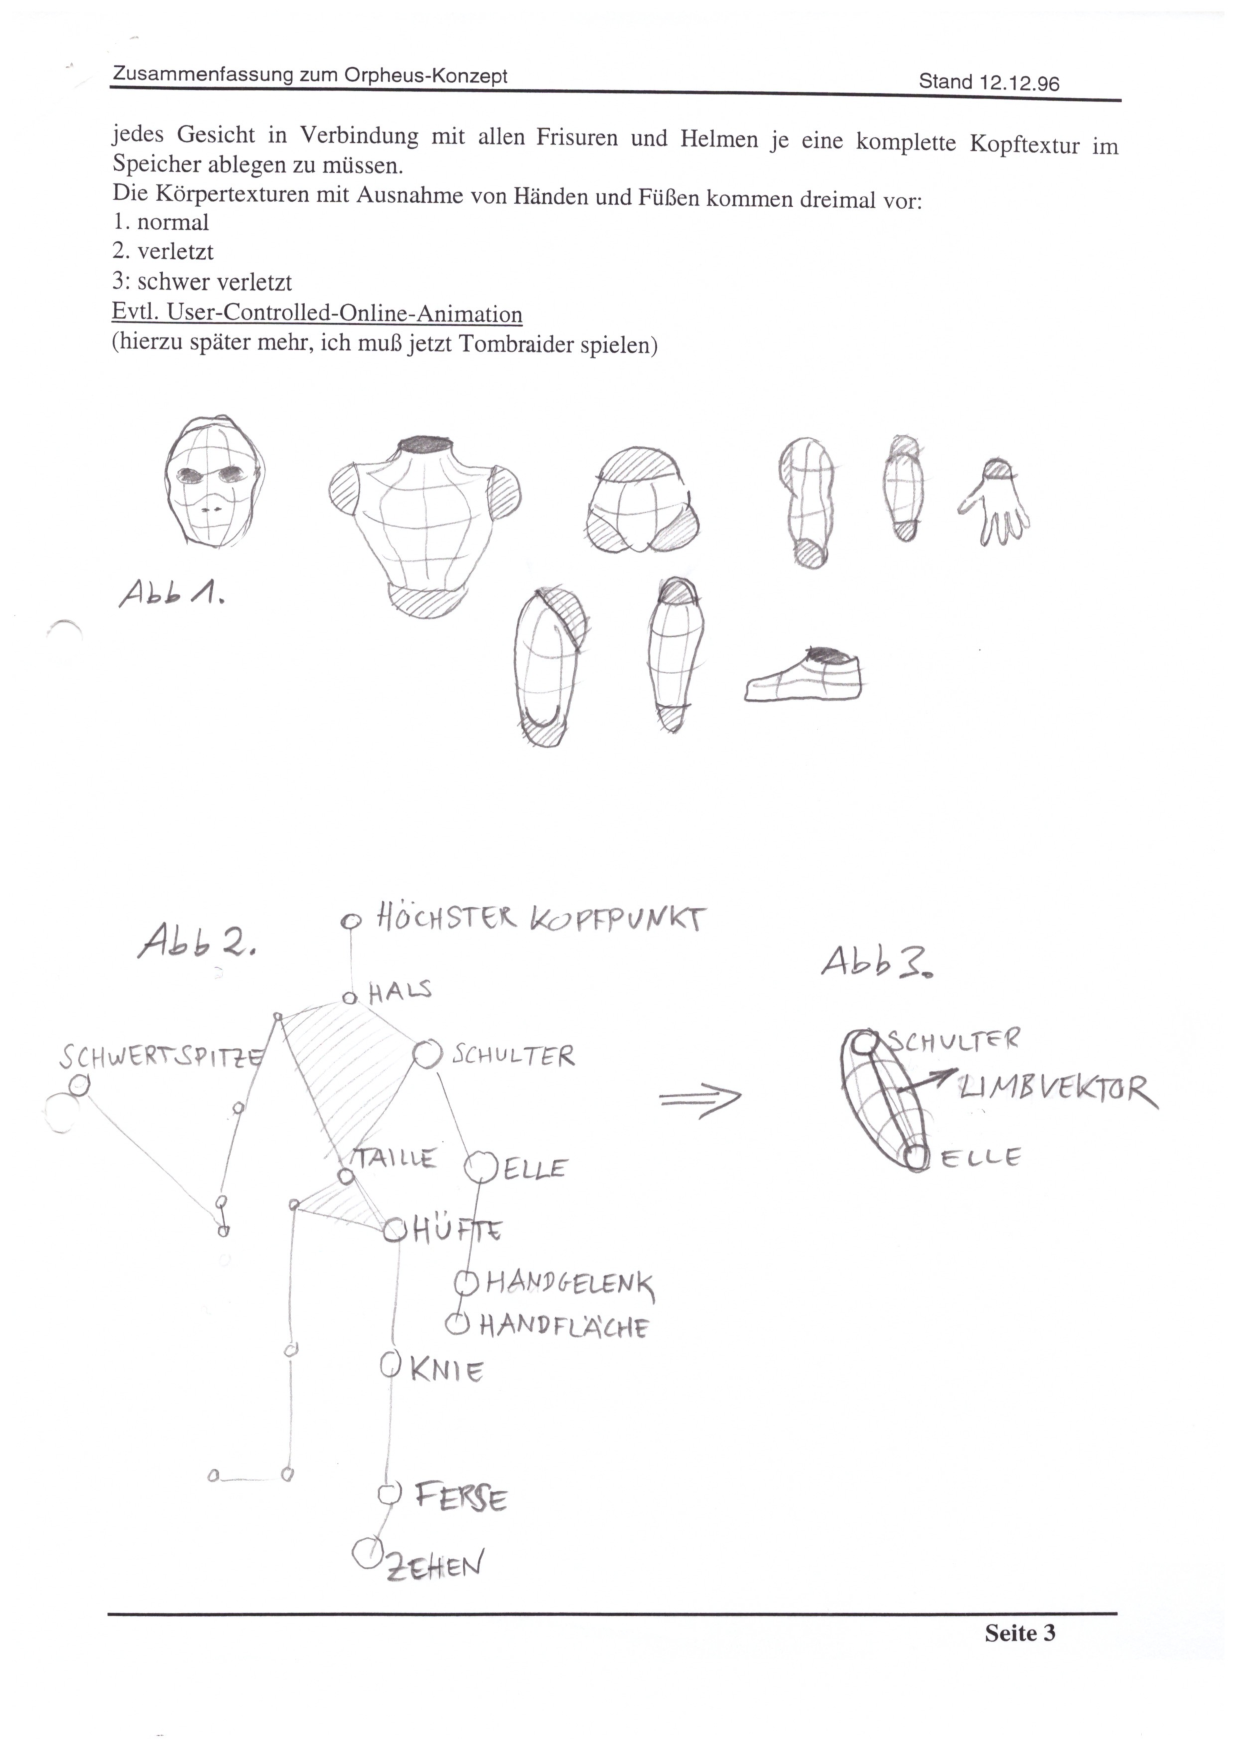
\includegraphics[scale=0.5]{orpheus_spielfigurenanimation.pdf}}
   \caption{Ausschnitt aus \enquote{Zusammenfassung zum Orpheus-Konzept}}
   \label{fig:orpheus_spielfigurenanimation}
\end{figure}


%%%%%%%%%%%%%%%%%%%%%%%%%%%%%%%%%%%%%%%%%%%
% ORPHEUS – DARSTELLUNG – BEWEGUNGSUMFANG %
%%%%%%%%%%%%%%%%%%%%%%%%%%%%%%%%%%%%%%%%%%%
\subsection{Bewegungsumfang}\label{sec:orpheus_darstellung_bewegungsumfang}
Auf der ersten Seite von \enquote{Orpheus -- Bewegungen} finden wir insgesamt 17 Spiegelstriche mit geplanten Animationen und der Information, in wieviele Phasen diese jeweils unterteilt sein sollten.\footnote{Einen Vergleich zu den im fertigen Spiel enthaltenen Animationen ermöglicht die \textit{Marvin-Datenbank}, deren Zweck es ist, den Testmodus von Gothic (den sogenannten \textit{Marvin Mode}) zu dokumentieren (vgl. \autocite{sillus_marvin_2020}).}
An oberster Stelle steht beispielsweise \enquote{Einhand Angriff × [2] (7 Pha)}.
Geplant waren also vermutlich zwei Varianten eines Angriffs mit einer einhändig geführten Waffe (vielleicht ein Streich von links nach rechts und ein zweiter von rechts nach links), die jeweils sieben Animationsphasen umfassen sollten.
Daneben gibt es hier unter anderem \enquote{Zweihand Angriff}, \enquote{Armbrust}, \enquote{Bogen}, \enquote{getroffen werden} und \enquote{umfallen}, \enquote{mag. offensiv} und \enquote{mag. defensiv} sowie \enquote{stehen}, \enquote{gehen}, \enquote{geduckt gehen}, \enquote{rennen}, \enquote{klettern}, \enquote{Schwimmen} und \enquote{Springen (gehend wie stehend)}, aber auch \enquote{rennend}.

Auf den folgenden -- wahrscheinlich später entstandenen -- drei Seiten wird diese Liste dann unter anderem um \enquote{Dialoggesten} ergänzt und wesentlich ausdifferenziert, insbesondere für Kampfanimationen und Bewegungen mit gezogener Waffe.
Hier tauchen dann neben dem Ziehen der Waffe (\enquote{Draw}, \enquote{Bogen ziehen}, \enquote{Armbrust anlegen}) sowie der \enquote{At[tacke]} und der \enquote{Pa[rade]} unter anderem auch \enquote{Kür}, \enquote{Unterschläge} sowie \enquote{Ruhehaltung} beziehungsweise \enquote{Standpose} auf und das Bewegungsrepertoire wird um das Umdrehen (\enquote{Turn}) sowie um Seitwärtsbewegungen (\enquote{Strafe}) erweitert.
Ein Stichwort fällt besonders ins Auge:
An drei Stellen notiert Mike Hoge \enquote{Threaten \& Kill, Xena-Move}.
Dabei bezieht er sich vermutlich auf die kampferprobte Protagonistin der zwischen 1995 und 2001 gedrehten Fernsehserie \textit{Xena -- Die Kriegerprinzessin}, wobei nicht klar ist, welcher ihrer \enquote{Moves} hier gemeint ist. % Mike Hoge fragen.

Eine ähnliche Auflistung geplanter Animationen finden wir in der \enquote{Zusammenfassung} am Ende des Abschnitts zur \enquote{\uline{Spielfigurenanimation}} (siehe \autoref{sec:orpheus_darstellung_animation}).
Dort gibt es eine Liste, in der insgesamt 48 \enquote{\textit{Geplante Menschenanimationen}} aufgeführt werden:
\enquote{stehen}, \enquote{gehen}, \enquote{rennen}, \enquote{strafen}, \enquote{rückwärts gehen}, \enquote{umdrehen}, \enquote{ducken}, \enquote{im Stand springen}, \enquote{nach vorne springen}, \enquote{rennend springen}, \enquote{an Wand klettern}, \enquote{an Seil klettern}, \enquote{seitlich klettern}, \enquote{an Vorsprung hochziehen}, \enquote{an Vorsprung herunterlassen}, \enquote{getroffen werden}, \enquote{getroffen stürzen}, \enquote{wieder aufstehen}, \enquote{Axt vom Rücken nehmen}, \enquote{Schwert ziehen}, \enquote{schwimmen}, \enquote{tauchen}, \enquote{Gegenstand ablegen}, \enquote{Gegenstand aufnehmen}, \enquote{geben und nehmen}, \enquote{Tür öffnen und schließen}, \enquote{umsehen}, \enquote{Faustschlag}, \enquote{Treten}, \enquote{werfen}, \enquote{schleudern}, \enquote{Schwertstreich}, \enquote{zweihändiger Schwertstreich}, \enquote{Schildparade}, \enquote{linker Schwertstreich}, \enquote{Befreiungsschlag}, \enquote{Drehschlag (Kopf ab)}, \enquote{Bogenschießen}, \enquote{Armbrustschießen}, \enquote{tödlicher Pfeil}, \enquote{tödlicher Hieb}, \enquote{offensive Magie}, \enquote{defensive Magie}, \enquote{fliegen}, \enquote{geduckt gehen}, \enquote{kriechen}, \enquote{von Stand in Hocke} und \enquote{von Hocke auf Boden}.
Auch hier finden wir stellenweise -- nachträglich mit einem Bleistift ergänzt -- Informationen zu den geplanten Animationsphasen; neben dem \enquote{Schwertstreich} ist beispielsweise -- konsistent mit dem \enquote{Einhand Angriff} in \enquote{Orpheus -- Bewegungen} -- eine \enquote{7} notiert.


%%%%%%%%%%%%%%%%%%%%%%%%%%%%%%%%%%%%%%%%%%%
% ORPHEUS – DARSTELLUNG – FIGURENVIELFALT %
%%%%%%%%%%%%%%%%%%%%%%%%%%%%%%%%%%%%%%%%%%%
\subsection{Figurenvielfalt}\label{sec:orpheus_darstellung_figurenvielfalt}
In der \enquote{Zusammenfassung} werden unter den Überschriften \enquote{\uline{Diverse Meshes}} und \enquote{\uline{Texturen}} Ideen aufgeführt, die die technisch effiziente Ermöglichung einer möglichst große Figurenvielfalt behandeln.

Zunächst sollten, wie wir unter \enquote{\uline{Diverse Meshes}} erfahren, die als Meshes abgespeicherten Limbs (siehe \autoref{sec:orpheus_darstellung_animation}) in verschiedenen Formen verfügbar sein und sich beliebig am Gelenk-Animations-Modell kombinieren lassen:
\enquote{Jedes Limb-Mesh kommt in mehreren Ausführungen vor.
Somit kann man verschiedene Köpfe, Oberkörper, etc. in dasselbe GAM einhängen.}
In einer Tabelle sind verschiedene mögliche Formen für die jeweiligen Limbs (\enquote{Kopf}, \enquote{Oberkörper}, \enquote{Unterleib}, \enquote{Oberarm}, \enquote{Unterarm}, \enquote{Hand}, \enquote{Oberschenkel}, \enquote{Unterschenkel} und \enquote{Fuß}) gesammelt.
Für den \enquote{Kopf} sind das beispielsweise \enquote{Visierhelm, Kettenkappe, Kapuze, Hut, lange Haare, kurze Haare, Glatze} und für den \enquote{Unterleib} sind es \enquote{Hose, Röckchen}.
In einer Anmerkung notiert Mike Hoge: \enquote{\textit{Die Hand bildet eine Ausnahme, da ihr Mesh nicht vom Zustand, sondern von den Aktionen der Figur beeinflußt wird}}.
Dementsprechend finden wir hier die Varianten \enquote{offen, geschlossen, hält sich fest}.
Die \enquote{\uline{Vorteile}} liegen auf der Hand:

\begin{quote}
   Durch das Baukastensystem wird durch Kombinationen große Figurenvielfalt erreicht.
   Würden alle Figuren als Ganzkörpermesh abgelegt, würden z.\,B. in einer Stadt nur wenige Menschen mit verschiedenen Meshes herumlaufen.
   Vor allen Dingen beim Kopf wäre dies tragisch.
   Mit dem Baukastensystem kann man Köpfe mit verschiedenen Frisuren oder Helmen mit gleichen Körpern kombinieren, und erhält so (in Verbindung mit unterschiedlichen Texturen) verschiedene Figuren.
\end{quote}

Für jede Ausführung der Limb-Meshes sollte es dann \enquote{individuell auf das entsprechende Limb zugeschneidert[e]} Texturen geben, wodurch sich \enquote{auch hier (durch unterschiedliche Texturierung gleicher Meshes) durch das Baukastensystem Vielfalt erzeugen} lässt, wobei zusätzlich alle \enquote{Körpertexturen mit Ausnahme von Händen und Füßen} in drei unterschiedlichen Varianten vorkommen sollten: \enquote{normal}, \enquote{verletzt} und \enquote{schwer verletzt}.
Aus Effizienzgründen sollten Texturen außerdem kombinierbar sein:

\begin{quote}
   Ein Limb kan [sic] mit zwei verschiedenen Texturen belegt werden.
   Bevor die Kopftextur auf das Kopf-Limb gemappt wird, wird diese aus Gesichtstextur und Kopftextur zusammengesetzt, um nicht für jedes Gesicht in Verbindung mit allen Frisuren und Helmen je eine komplette Kopftextur im Speicher ablegen zu müssen.
\end{quote}

Damit \enquote{bei Kamerafahrten nahe an die Figur keine Pixelhaufen als Gesicht entstehen}, sollten zumindest die Kopftexturen außerdem \enquote{als größere Grafiken abgelegt} werden.
Bei den Texturen für andere Limbs wäre das vernachlässigbar: \enquote{Beim Oberkörper ist dieser Effekt nicht so schlimm.}


%%%%%%%%%%%%%%%%%%%%%%%%%%%%%%%%%%%%
% ORPHEUS – DARSTELLUNG – INVENTAR %
%%%%%%%%%%%%%%%%%%%%%%%%%%%%%%%%%%%%
\subsection{Inventar}\label{sec:orpheus_darstellung_inventar}
Während sich der Großteil von \enquote{\uline{\textsc{Orpheus} -- Interface}} mit Fragen der spielerischen Möglichkeiten sowie der Steuerung befasst (siehe \autoref{sec:orpheus_mechanik_möglichkeiten}), gewährt die letzte der sieben Seiten Einblick in eine frühe Vision des Inventars.\footnote{Bereits auf der vorherigen Seite wird eine Reihe kleinerer Raster dargestellt, bei denen es sich um verschiedene Ideen für ein Inventar handeln könnte.}
Drei kleine, untereinander gezeichnete und von \enquote{1} bis \enquote{3} nummerierte Skizzen (siehe \autoref{fig:orpheus_inventar} oben) illustrieren hier den Übergang von der Spiel- zur Inventar\-ansicht.
Den Ausgangspunkt bildet die erste Skizze, in der wir die Spielfigur aus der Verfolgerperspektive (siehe \autoref{sec:orpheus_darstellung_kamera}) im Zentrum des Bildschirms sehen.
In der zweiten Skizze wird dann die \enquote{Inventory-Anim[ation]} dargestellt; beim Öffnen des Inventars hätte sich die Kamera in einem Halbkreis um die Spielfigur herum bewegen sollen, so dass man sie am Ende von vorne sieht.
Die Figur \enquote{Steckt [ihre] Waffen weg} und wäre am Ende der Kamerafahrt, wie die dritte Skizze zeigt, nicht mehr zentriert dargestellt, sondern an den linken Bildschirmrand verschoben, so dass rechts von ihr ausreichend Platz für die Darstellung des Inventars bleibt.
Im nun offenen Inventarbildschirm hätte wir also ein aktuelles \enquote{ingame \uline{pic}} unserer Figur sehen sollen, wobei offen bleibt, ob sich das Inventar -- wie im finalen Gothic -- über die weiterhin in Bewegung befindliche Spielwelt hätte legen oder -- wie das Wort \enquote{\uline{pic}} implizieren könnte -- ein statische Abbildung hätte zeigen sollen.

In einer separaten Skizze ist die Struktur des Inventars selbst dargestellt (siehe \autoref{fig:orpheus_inventar} unten).
Am linken Bildschirmrand befindet sich die Spielfigur, rechts neben ihr auf dem Boden steht etwas, das einen Rucksack darstellen könnte (und das auch schon in der oben erwähnten dritten Skizze erkennbar zu sein scheint).\footnote{Tatsächlich wurde während der Entwicklung ein Rucksack -- beziehungsweise, der Optik nach, eine Art Kiepe -- implementiert, der von Figuren getragen werden konnte, wie in Version 0.94k zu sehen ist; vgl. bspw. \autocite{alpha_backpack_2023}.}
Rechts davon werden vier vertikale Balken angedeutet, die den Bildschirm in voller Höhe ausfüllen.
Im -- von links gezählt -- zweiten Balken deutet jeweils ein Pfeil an den oberen und ein Pfeil an den unteren Bildschirmrand; im vierten Balken wiederum ist ein Pfeil am unteren Bildschirmrand mit \enquote{\textsc{Cont[inue]}} beschriftet.
Die Balken hätten sich also wahrscheinlich nach oben und unten durchblättern lassen sollen -- und zwar mit den entsprechenden Pfeiltasten.
Darauf deutet eine Notiz an anderer Stelle auf dieser Seite hin:
In einer von späterer Hand wieder durchgestrichenen Sammlung an Stichpunkten zur Waffenauswahl ist \enquote{$_{\downarrow}^{\uparrow}$ Inventory Scroll} vermerkt. % Verweis Steuerung

In den ersten drei Balken findet sich oberhalb der Bildschirmmitte jeweils ein Symbol, das stellvertretend für die in diesem Balken gesammelte Art von Gegenständen stehen könnte:
Ein Schlüssel, ein Schwert und ein Kleidungs- oder Rüstungsteil für den Oberkörper, wobei das Schwert und das Kleidungs- oder Rüstungsteil jeweils in einen eigenen Kasten eingefasst ist.
Der vierte Balken scheint zweigeteilt zu sein:
In seiner oberen Hälfte werden vier Kleidung- oder Rüstungsteile dargestellt und von einer Wellenlinie umschlossen:
Ein Teil für den Kopf, eines für den Oberkörper, eines für die Beine sowie eines für die Füße.
Zwischen den Teilen für Kopf und Oberkörper ist etwas nach rechts versetzt ein kleiner, teilweise schraffierter \enquote{\textsc{Balken}} platziert, dessen Funktion nicht ersichtlich ist; vielleicht hätte er den Zustand eines Ausrüstungsteils indizieren sollen. % Mike Hoge fragen.
In der unteren Hälfte sind die gleichen vier Teile in unterschiedlicher Reihenfolge (Oberkörper, Beine, Kopf, Füße) noch einmal abgebildet, auf der rechten Seite eingefasst von einer geschweiften Klammer, neben der \enquote{\uline{Scroll}} notiert ist.
Am unteren Ende dieses Balkens befindet sich der oben bereits erwähnte abwärtsdeutende Pfeil, unter dem \enquote{\textsc{Cont}} geschrieben steht.
In der unteren rechten Ecke der Skizze steht in einem kleinen Kasten \enquote{\textsc{Shortsword}}; vielleicht hätte hier die Bezeichnung des jeweils im Fokus befindlichen Gegenstands erscheinen sollen. % Mike Hoge fragen.
In einem etwas oberhalb der Bildschirmmitte befindlichen kleinen Kasten, ebenfalls am rechten Rand der Skizze, steht diagonal \enquote{\textsc{Trap}}; eventuell hätte hier eine aktuell ausgerüstete Falle angezeigt werden sollen. % Verweis Fallensteller
Auf gleicher Höhe ist rechts außerhalb der Umrandung ein weiterer Kasten eingezeichnet, in dem -- ebenfalls diagonal -- \enquote{\textsc{Log}} geschrieben steht; rechts neben dem Kasten prangt ein dünnes Ausrufezeichen.
Beides -- Kasten und Ausrufezeichen -- wird von einer Umrahmung an den rest der Skizze angeschlossen, so dass es wie ein seitlicher Register-Reiter wirkt; eventuell hätte man von hieraus auf das Tagebuch wechseln können sollen.

\vfill
\begin{figure}[p]
   \centering
   \fbox{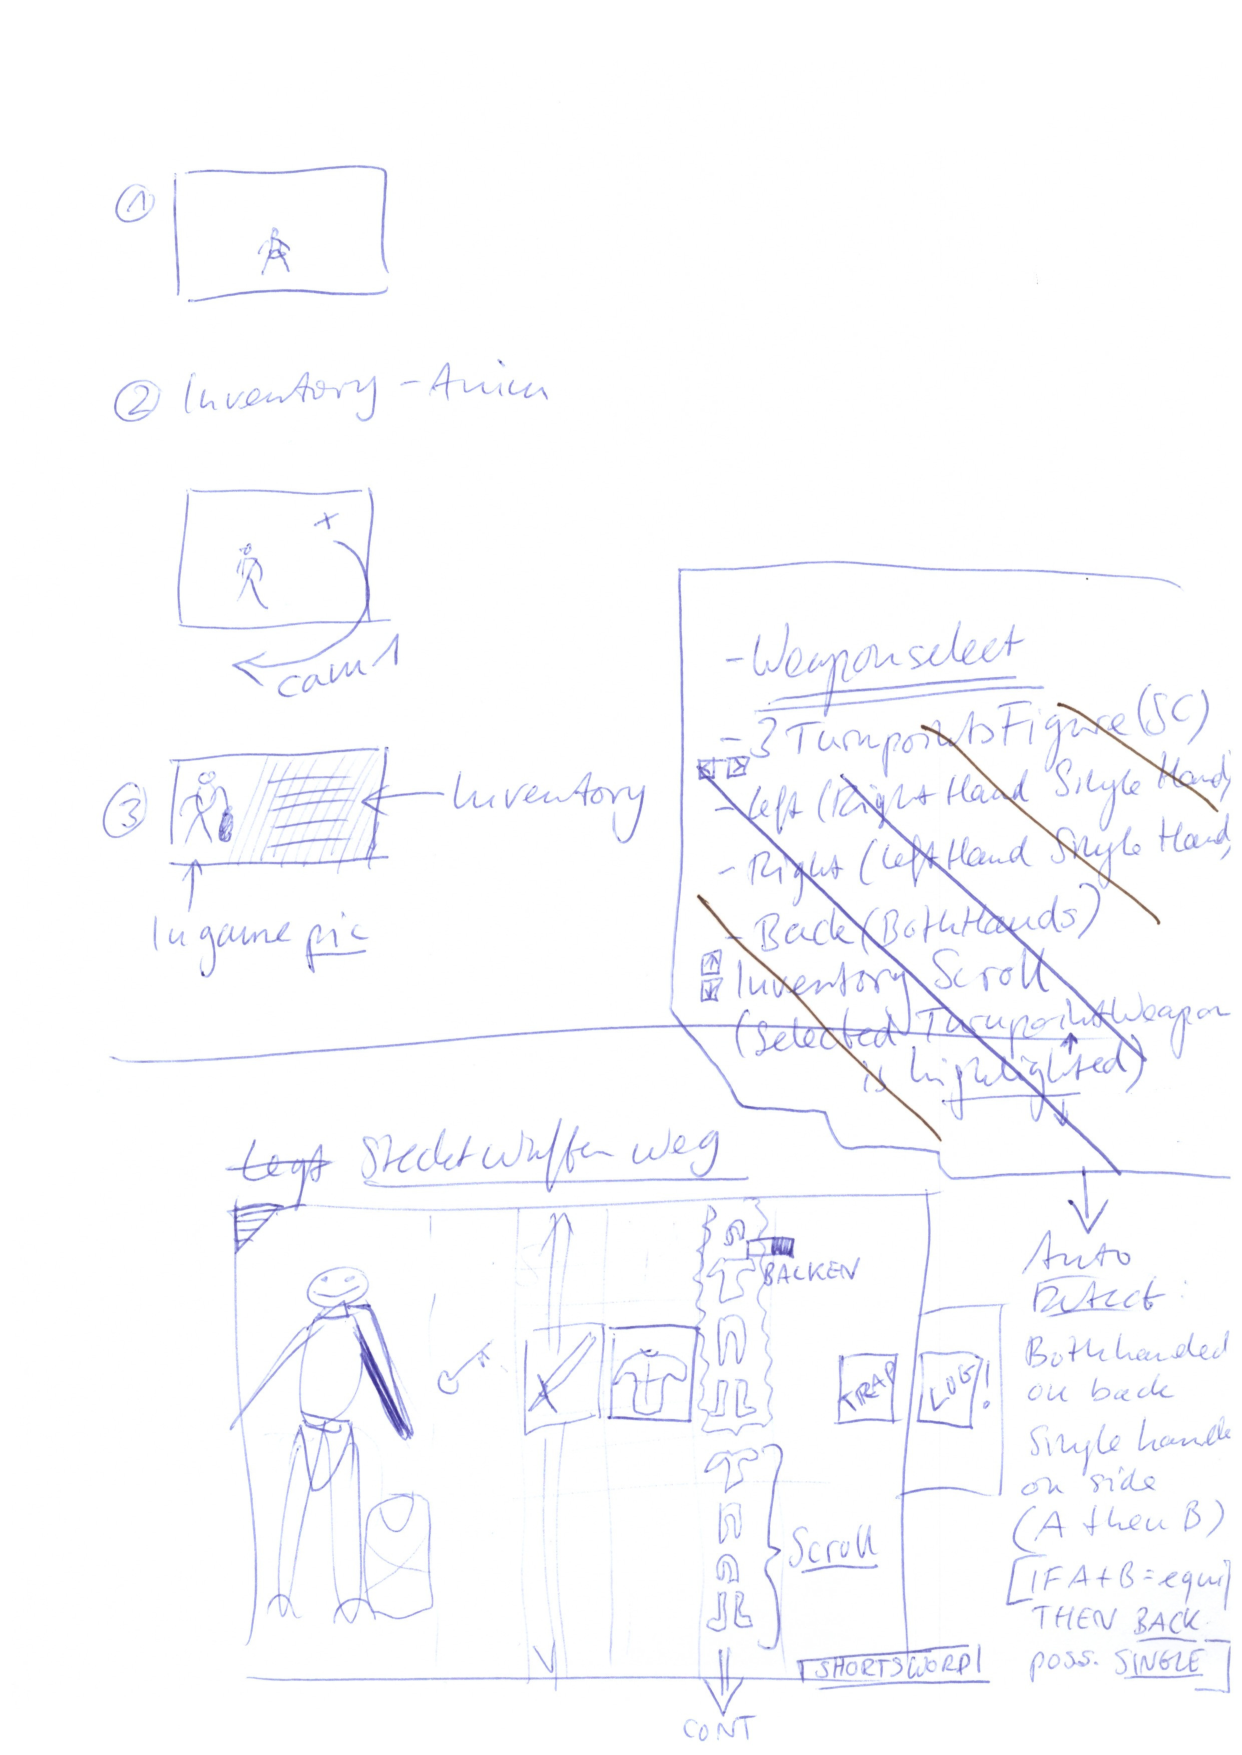
\includegraphics[scale=0.5]{orpheus_inventar.pdf}}
   \caption{Ausschnitt aus \enquote{\uline{\textsc{Orpheus} -- Interface}}}
   \label{fig:orpheus_inventar}
\end{figure}


%%%%%%%%%%%%%%%%%%%%%%%%%%%
% ORPHEUS – SPIELMECHANIK %
%%%%%%%%%%%%%%%%%%%%%%%%%%%
\section{Spielmechanik}\label{sec:orpheus_mechanik}
Einige der oben genannten Dokumente befassen sich im weitesten Sinne mit spielmechanischen und steuerungsbezogenen Fragen, nämlich weite Teile von \enquote{Orpheus -- Interface} sowie die Notizen zur Kampfsteuerung.
Auch im Konvolut \enquote{Orpheus. B -- Scribbles} finden sich relevante Stichpunkte.

\enquote{Spielmechanik} verstehe ich dabei relativ weit gefasst als die Menge an Möglichkeiten, die Spieler:innen zur Verfügung gestellt wird, um mit Spielelementen interagieren zu können.\autocite[255]{jaervinen_games_2008}
Diese Möglichkeiten lassen sich in der Regel, wie wir unten sehen werden, durch Verben beschreiben.\autocite[263]{jaervinen_games_2008}

Wir werfen zuerst einen Blick darauf, welche Möglichkeiten Spieler:innen eröffnet werden sollten (\autoref{sec:orpheus_mechanik_möglichkeiten}) und schauen uns anschließend an, wie sich das Ganze hätte steuern lassen sollen (\autoref{sec:orpheus_mechanik_steuerung}).


%%%%%%%%%%%%%%%%%%%%%%%%%%%%%%%%%%%%%%%%%%%
% ORPHEUS – SPIELMECHANIK – MÖGLICHKEITEN %
%%%%%%%%%%%%%%%%%%%%%%%%%%%%%%%%%%%%%%%%%%%
\subsection{Spielerische Möglichkeiten}\label{sec:orpheus_mechanik_möglichkeiten}
Auf der ersten Seite von \enquote{\uline{\textsc{Orpheus} -- Interface}}\autocite[Vgl.][]{orpheus_interface} (siehe \autoref{sec:orpheus_darstellung_inventar}) begegnen uns an oberster Stelle drei nummerierte Stichpunkte mit grundlegende Designentscheidungen:
\enquote{\uline{Outside View Only}},\footnote{Das steht in Konflikt mit den Ausführungen unter \enquote{\uline{Spielansicht}} in der \enquote{Zusammenfassung}, wonach auch eine Egoperspektive vorgesehen war (siehe \autoref{sec:orpheus_darstellung_kamera}).} \enquote{\uline{Tastatur Only} (evtl Maus Inventory \& \enquote{\uline{Fernklick}} Unterstützung)} sowie \enquote{Items = VOBs}.\footnote{\enquote{VOB} steht hier für \enquote{Virtuelles Objekt}; zur Rolle von VOBs bei Gothic \autocite[vgl.][]{wiki_vob}.}
Alle drei Punkte haben sich als für die Entwicklung von Gothic maßgeblich herausgestellt:
Den Namenlosen Helden sehen wir immer aus der Verfolgerperspektive, die Steuerung unterstützt zwar Mauseingabe, bleibt in der Hauptsache aber auf die Tastatur fokussiert, und alle Gegenstände, die wir in der Spielwelt finden können, sind in der Engine als virtuelle Objekte angelegt.

Unter diesen drei wegweisenden Stichpunkten folgt dann eine von \enquote{a} bis \enquote{p} reichende Liste mit Möglichkeiten, die Spieler:innen haben sollten:
\enquote{div[erse] Schläge}, \enquote{Zielen \& Schießen}, \enquote{Spell Selection}, \enquote{klettern}, \enquote{Springen}, \enquote{Türen öffnen/Truhe öffnen}, \enquote{Schloß knacken}, \enquote{ansehen}, \enquote{VOB verschieben}, \enquote{in VOB verstecken}, \enquote{Party NSC lenken}, \enquote{Battle Mode}, \enquote{reden}, \enquote{aufheben}, \enquote{Inventory} und \enquote{weglegen}.
Das meiste davon ist am Ende auch umgesetzt worden; nur bei vier Punkten -- \enquote{VOB verschieben}, \enquote{in VOB verstecken}, \enquote{Party NSC lenken} und \enquote{Battle Mode} -- gibt es nennenswerte Abweichungen.

Nachdem Mike Hoge sich zu dieser Zeit noch die Frage \enquote{sollen \uline{alle} mögl. \uline{verschiebbar} sein?}\autocite[S.~3]{orpheus_interface} notiert hatte, ist \enquote{VOB verschieben} im fertigen Spiel -- wenn überhaupt -- nur noch als einzelnes, für Spieler:innen irrelevantes Artefakt vorhanden:
In der Klosterruine gibt es eine freistehende Säule, die sich zwar nicht wirklich verschieben, aber zumindest umwerfen lässt -- wobei sie dann auch noch in die falsche Richtung fällt.
Es scheint offensichtlich, das sie als improvisierte Brücke zur Überwindung eines Abgrunds dienen sollte.
Statt über den Abgrund fällt sie aber, wenn man sie umstößt, vom Abgrund fort.
Ob das schon als \enquote{verschieben} zählen darf, ist freilich diskutabel.
An die Idee, zum Beispiel einen \enquote{Schrank [$\ldots$] verschieben}\autocite[S.~3]{orpheus_interface} zu können, reicht es jedenfalls nicht mehr heran.

Ähnlich sieht es für den Stichpunkt \enquote{in VOB verstecken} aus:
Vereinzelt finden wir in der Spielwelt noch Fässer\footnote{Ein Objekt, das uns an verschiedenen Stellen in den Notizen begegnet, vgl. \autocite[S.~19]{orpheus_b_scribbles}, \autocite[S.~6]{orpheus_interface}.} -- eines im Alten Lager und zwei in der Alten Miene --, in denen sich unser Namenloser Held verstecken kann.
Eine darüberhinausgehende spielrelevante Funktion erfüllen sie aber nicht.

Bei Gothic steht außerdem nur eine Spielfigur im Fokus und damit keine klassische Party, die sich aus verschiedenen Charakteren zusammensetzt.
Zwar gibt es vereinzelt Begleiter, mit denen man kurzfristig gemeinsam durch die Spielwelt streifen kann, steuern lassen sich diese allerdings -- wenn man von dem Zauber \enquote{Kontrolle} einmal absieht -- nicht. % Prüfen, ob das geht
\enquote{Party NSC lenken} ist im Laufe der Entwicklung also auch unter den Tisch gefallen.
Darauf, dass die Möglichkeit einer Party aber ernsthaft in Erwägung gezogen wurde, deuten einige weitere Notizen in \enquote{Orpheus -- Interface} hin.
\enquote{Bis zu 4 Party NSCs}\footnote{\autocite[S.~5]{orpheus_interface}. An anderer Stelle ist von \enquote{2 Slots (1 + 1)} die Rede (\autocite[S.~7]{orpheus_b_scribbles}).} sollte es geben.
Diese \enquote{Kontrollierte[n] NSCs [sollten] \uline{farblich} gekennzeichnet}\autocite[S.~5]{orpheus_interface} sein und sich über eine Reihe an Befehlen steuern lassen.
In einer kleinen Skizze sind dafür vier nebeneinanderliegende Tasten eines \enquote{Pop Up Menu[s]} mit \enquote{follow}, \enquote{wait}, \enquote{action} und \enquote{attack} beschriftet.\autocite[S.~3]{orpheus_interface}
An anderer Stelle finden wir eine abweichende Variante mit vier verschiedenen Knöpfen:
Über den \enquote{\uline{1. Button}} sollte ein kontrollierter Charakter dazu aufgefordert werden können, zu \enquote{Warte[n]} oder zu \enquote{Folge[n]}.
Eine dritte Option, nämlich ihn \enquote{\sout{Fliehe}[n]} zu lassen, ist hier durchgestrichen.
Über einen \enquote{\uline{2. Button}} sollte er dazu aufgefordert werden können, eine \enquote{Aktion} auszuführen, beispielsweise -- bezogen auf eine Tür -- \enquote{Lockpick} oder \enquote{Einrennen}.
Über einen \enquote{\uline{3. Button}} hätte man über \enquote{Kampf/Sparflamme} entscheiden können sollen, also wahrscheinlich darüber, ob der kontrollierte Charakter mit gezogener Waffe kampfbereit sein soll oder nicht.
Die Partymitglieder \enquote{kämpfen bis 15\%} ihrer Lebensenergie, hätten aber \enquote{\uline{Keine} selbstständige Aggression gegen andere NSCs}.
Über einen \enquote{General Button} schließlich hätte sich ein \enquote{Kriegsrat} der Party einberufen lassen sollen.
Diese Befehle hätten sich wahrscheinlich jeweils auf ein einziges Mitglied der Gruppe beziehen sollen.
Darauf könnte zum einen hindeuten, dass die Notiz so aussieht, als sollten die drei Buttons unter dem Balken für Lebensenergie erscheinen, der üblicherweise erscheint, wenn man sich einem NSC (oder einem Monster) zuwendet.
Außerdem sind zwei weitere -- danach wieder durchgestrichene -- Ideen für einen \enquote{\sout{General Button 2}} sowie einen \enquote{\sout{General Button 3}} notiert.
Mit ersterem hätte man zwischen \enquote{\sout{Alle Warten/Alle Folgen/Alle Kampf}} und mit zweiterem zwischen \enquote{\sout{Kampf/Alle Still}} umschalten können sollen;\autocite[S.~5]{orpheus_interface} \enquote{General} scheint sich also immer auf die ganze Gruppe zu beziehen.

Eine solche Party bringt andere spielmechanische Herausforderungen mit sich als ein einzelner Charakter:
Wenn unser Namenloser Held in Gothic stirbt, ist das Spiel zu Ende und wir müssen neu laden.
Aber wie geht man damit um, wenn nur ein Mitglied der Party stirbt?
\enquote{\textsc{Wie Wiederbelebung?}} fragt Mike Hoge an einer Stelle und notiert daneben, dass das über einen \enquote{\uline{Schrein}} geregelt werden könnte, der dem \enquote{Mafiabos} gehört.\autocite[S.~7]{orpheus_b_scribbles}
Die auf einer anderen Seite befindliche Notiz \enquote{\uline{1} XP Pool}\autocite[S.~8]{orpheus_b_scribbles} könnte sich wiederum darauf beziehen, dass Erfahrungspunkte nicht für jedes Partymitglied einzeln, sondern für die Gruppe als ganzes gezählt werden sollen.
Ein ähnliches Problem gibt es für die Objekte, die sich in der Spielwelt sammeln lassen:
\enquote{Individuell \textsc{oder} Gruppe} schreibt Mike Hoge unter der Überschrift \enquote{\uline{Besitzflag}}.
Es lässt sich vermuten, dass jedes Objekt entweder als Besitz eines Charakters oder als das der Party ausgewiesen werden sollte, wobei gilt:
\enquote{08/15 Items haben Gruppenflag.}\autocite[S.~9]{orpheus_b_scribbles}
Außerdem stellt sich -- darauf deutet der Stichpunkt \enquote{Partymitglied\_Bewegungs\_Spielraum}\autocite[S.~8]{orpheus_b_scribbles} hin -- die Frage, wie mit räumlicher Entfernung zwischen den einzelnen Partymitgliedern umgegangen werden soll.
Es gibt beispielsweise Überlegungen, dass die oben erwähnte Aufforderung \enquote{Folge} nicht funktionieren sollte, wenn sich ein Gruppenmitglied \enquote{außer Hörreichweite} befindet.
Weil das unter Umständen aber zu unpraktisch sein könnte, ist dazu in Klammern eine Alternative notiert:
\enquote{evtl Telepath. Kommunikation}.\autocite[S.~5]{orpheus_interface}
Und was macht man, wenn sich ein Gruppenmitglied -- aber nicht der Spieler selbst -- an einem Ort aufhält, an dem etwas Wichtiges ausgelöst werden soll?
Der etwas kryptische Vermerk \enquote{Kritische Dialoge \textsc{nicht} Triggern wenn \uline{Party} $-$ NSC $=$ \uline{Mensch}!}\autocite[S.~9]{orpheus_b_scribbles} könnte unter Umständen so gelesen werden, dass ein wichtiger Dialog nicht ausgelöst werden soll, wenn Teile der Gruppe zwar am entsprechenden Ort sind, der menschliche Spieler (\enquote{NSC = Mensch}) aber fehlt (\enquote{$-$}); wobei man freilich darüber hinwegsehen müsste, dass \enquote{NSC} eigentlich einen Charakter beschreibt, der nicht der Spieler ist.

Neben \enquote{VOB verschieben}, \enquote{in VOB verstecken} und \enquote{Party NSC lenken} bleibt dann noch der \enquote{Battle Mode}, wobei nicht unmittelbar klar ist, was sich die Entwickler zu diesem Zeitpunkt darunter vorgestellt haben.
Bei der Erwähnung eines solchen Kampfmodus mag einem zum Beispiel der unter anderem in JPRGs bis heute tradierte Kampfbildschirm in den Sinn kommen, in dem das (in der Regel rundenbasierte) Geschehen oft abstrahiert aus einem Blick von der Seite dargestellt wird, wobei sich die Kontrahenten beispielsweise am linken und rechten Rand des Bildschirms oder diagonal gegenüberstehen.\footnote{Ein frühes -- vielleicht sogar das erste -- Beispiel für eine Kampfansicht, in der sich die Parteien links und rechts gegenüberstehen, stellt das 1987 in Japan und 1990 in den Vereinigten Staaten erschienene \textit{Final Fantasy} dar. Eine diagonale Gegenüberstellung findet sich etwa in dem 1993 erschienenen \textit{Ogre Battle -- The March of the Black Queen}. Daneben gibt es noch die frontale Darstellung der Gegner, entweder aus der Egoperspektive des Spielers, wie etwa im 1986 veröffentlichten \textit{Dragon Quest}, oder über die Schulter der Spielfiguren, wie beispielsweise im 1993 erschienenen \textit{Lufia \& the Fortress of Doom}. Diese Formen eines separaten Kampfbildschirms haben sich bis heute erhalten, etwa im 2016 erschienenen \textit{Persona 5} oder im 2018 erschienenen \textit{Octopath Traveler}.}
Und tatsächlich sehen wir in einer frühen Entwicklungsversion von Gothic, dass sich die Kamera im Falle eines Kampfes zur Seite bewegt und das Geschehen aus einer statischeren Perspektive zeigt, die nicht mehr strikt dem Charakter folgt, sondern sich nur verschiebt, wenn dieser sich hinreichend weit von seiner ursprünglichen Position entfernt.\footnote{Das ist der Fall in Version 0.56c; vgl. bspw. \autocite[Min.~5:11]{alpha_features_2023}.}
Generell haben die frühen Überlegungen zum Kampf einen etwas taktisch anmutenden Charakter.
In \enquote{Orpheus -- Interface} ist die Idee festgehalten, dass man nach dem \enquote{Ausholen} (über \enquote{Fire}) mit \enquote{$\leftarrow$} und \enquote{$\rightarrow$} ein Ziel auswählen (\enquote{Select Target}), sich diesem dann mit \enquote{$\uparrow$} und \enquote{$\downarrow$} \enquote{nähern/entfernen} und schließlich über eine Auswahl zwischen \enquote{1} und \enquote{9} auf dem Ziffernblock eine Angriffsform auswählen kann (\enquote{Select Blow}).\autocite[S.~2]{orpheus_interface}
Die Notizen zur Kampfsteuerung lesen sich ähnlich taktisch.
Zentral ist bei den dort festgehaltenen Überlegungen die Distanz zum Gegner und wie sich diese durch die eigene Bewegung (etwa durch einen Angriff mit Ausfallschritt nach vorne oder durch eine Parade mit Schritt nach hinten) und die Bewegung des Gegners (etwa durch ein Zurückweichen beim Getroffenwerden) verändert.\autocite[Vgl.][S.~1--3]{orpheus_kampfsteuerung}
In einer Tabelle ist minutiös festgehalten, welche Art von Angriff welche Auswirkungen auf einen Gegner in welcher Distanz haben soll.\footnote{Vgl. \autocite[S.~4--5]{orpheus_kampfsteuerung}.}
Dabei wird unterschieden zwischen vier für den Nahkampf relevanten Distanzen, vier möglichen Tastatureingaben (\enquote{\textsc{Ctrl}} in Kombination mit \enquote{$\uparrow$}, \enquote{$\rightarrow$}, \enquote{$\leftarrow$} oder \enquote{$\downarrow$}) sowie einem Angriff mit der \enquote{Faust} oder mit einer von drei Waffen (\enquote{Dolch}, \enquote{Schwert} und \enquote{Zweihänder}), mit denen man entweder geübt oder ungeübt sein kann, was in einer Tabelle mit immerhin 112 Zellen resultiert.\autocite[S.~4]{orpheus_kampfsteuerung}


%%%%%%%%%%%%%%%%%%%%%%%%%%%%%%%%%%%%%%%
% ORPHEUS – SPIELMECHANIK – STEUERUNG %
%%%%%%%%%%%%%%%%%%%%%%%%%%%%%%%%%%%%%%%
\subsection{Steuerung}\label{sec:orpheus_mechanik_steuerung}
Gothic war schon immer für seine etwas eigenwillige Steuerung bekannt.
Petra Schmitz, die das Spiel vor seiner Veröffentlichung für die \textit{GameStar} bei einem Preview-Termin anspielen konnte, erinnert sich daran, wie schockiert sie davon war, dass das Spiel zu diesem Zeitpunkt keine Maussteuerung unterstütze.\autocite{schmitz_maussteuerung_2021}
Die oben erwähnte Notiz \enquote{\uline{Tastatur Only}}\autocite[S.~1]{orpheus_interface} (siehe \autoref{sec:orpheus_mechanik_möglichkeiten}) sollte bei der Entwicklung bis zum Schluss richtungsweisend bleiben.

Ein zentrales Element der Steuerung im finalen Gothic ist die Steuerungstaste (kurz Strg).
Während die Bewegung klassisch über die Tasten W, A, S und D funktioniert, gesellt sich Strg hinzu, wenn wir mit Elementen in der Spielwelt interagieren möchten.
Drücken wir beispielsweise -- während wir mit unserem namenlosen Helden einen Gegenstand oder eine Person anvisieren -- Strg und W, können wir etwa ein Objekt benutzen, einen Gegenstand aufsammeln, eine Truhe öffnen oder eine Person ansprechen.
In der Zeit von Orpheus sind solche Dinge noch auf verschiedene Tastenkombinationen verteilt.
\enquote{Fire + $\uparrow$} war für das \enquote{\uline{Manipulieren}} von Objekten in der Spielwelt (\enquote{Tür/Schrank/Truhe/Hebel/Knopf/Fackel}), \enquote{Fire + $\downarrow$} für das \enquote{\uline{Aufheben}} von Gegenständen (wobei man anschließend mit \enquote{up} oder \enquote{down} hätte entscheiden können sollen, ob man den Gegenstand ins Inventar aufnehmen oder \enquote{wieder weglegen} möchte), \enquote{Fire + $\leftarrow$} für das \enquote{\uline{Betrachten}} und \enquote{Fire + $\rightarrow$} für das \enquote{\uline{Reden}} gedacht.\autocite[S.~2]{orpheus_interface}
Daneben war \enquote{Alt} für \enquote{Springen/Klettern/in VOB verstecken} vorgesehen.\autocite[S.~3]{orpheus_interface}

Im fertigen Spiel machen wir uns durch Drücken der Leertaste Kampfbereit.
Diese Idee ist schon in \enquote{Orpheus -- Interface} angelegt, wo notiert ist, dass durch einmaliges Drücken das Schwert gezogen und durch zweimaliges Drücken der Bogen bereit gemacht werden sollte.\autocite[S.~2]{orpheus_interface}
Mit gezogener Waffe (oder gehobenen Fäusten, wenn wir keine Waffe ausgerüstet haben) können wir dann durch die Strg im Kombination mit W, A oder D angreifen, während uns Strg und S blocken lässt.
Diese Kombination von Steuerungs- und Richtungstasten geht -- wie wir oben im Zusammenhang mit der Tabelle gesehen haben -- ebenso auf diese frühe Phase zurück.
Den Notizen zur Kampfsteuerung zufolge sollte durch die Kombination von Strg und Pfeiltasten entweder unterschiedliche Gegner angegriffen oder verschieden Schwertstreiche auf den gleichen Gegner ausgeführt werden können.\footnote{Vgl. \autocite[S.~1--3]{orpheus_kampfsteuerung}; siehe auch \autocite[S.~4]{orpheus_interface}, wo wir ein Raster aus 3 × 3 Tasten finden, die in Kombination mit \enquote{Fire} jeweils unterschiedliche Aktionen im Kampf bewirken sollten. Von link nach Rechts sind das in der obersten Reihe \enquote{Tritt}, \enquote{Stechen} und Schlag von \enquote{Oben}, in der mittleren Reihe \enquote{L[inks] Seitlich [schlagen]}, \enquote{Barbarenschlag} und \enquote{R[echts] Seitlich [schlagen]} sowie in der unteren Reihe \enquote{L[inks] Rumgehen}, \enquote{Hinter Schlag} und \enquote{R[echts] Rumgehen}. Dieses Raster ist schon auf S.~1 hinter Punkt (a) \enquote{div[erse] Schläge} angedeutet.}

Die Notizen zur Auswahl von Zaubern wiederum sind etwas kryptisch.
Es scheint, als sei die erste Idee gewesen, dass man über eine Funktion zum Schnellzugriff mittels der Tabulatortaste auf verschiedene Gegenstände hätte zugreifen können sollen, wobei eines davon das Zauberbuch gewesen wäre (\enquote{QuickSlot2 $=$ SpellBook; $\rightleftarrows$<\textsc{tab}> $=$ Get\uline{QS2}items}).
Über \enquote{Fire} hätte sich dann ein Spruch aus dem Buch vorbereiten lassen sollen (\enquote{<Fire> $=$ \uline{Activate} [Bookmark] Spell}).
Darunter ist notiert, dass sich das Buch auch über die Eingabetaste hätte öffnen lassen (\enquote{<Return> $=$ Book $\Rightarrow$ Spell Select (Bookmark)}) und sich eine Auswahl an Zaubern unter Umständen auf den Nummernblock hätte legen lassen (\enquote{evtl. QuickChoiceSpells on Keypad 1--0}) sollen.
Es scheint damit so, dass man sich zuerst einen Zauber aus seinem Buch hätte zurechtlegen müssen, ehe man ihn dann -- in einem nächsten Schritt -- hätte wirken können.
Von späterer Hand sind allerdings zwei Notizen hinzugefügt worden, die darauf hinzudeuten scheinen, dass sich -- entweder auch oder stattdessen -- ohne den Umweg über das Zurechtlegen \enquote{\textsc{direkt aus} [dem] \textsc{Buch zaubern}} lassen sollte, indem man zunächst die Eingabetaste drückt, dann denn Zauber auswählt und ihn dann mit \enquote{Fire} wirkt (\enquote{<Return>$_{\downarrow}^{\uparrow}$<Fire>}).
Neben diesen Überlegungen zur Steuerung finden wir an dieser Stelle zwei generelle Gedanken zu Zaubern:
Sie sollten, erstens, einer \enquote{\textsc{\uline{logische}}[n] \textsc{\uline{Sortierung}}} folgen und, zweitens, sollte es \enquote{\textsc{wenig Sprüche auf einmal}} geben, die dafür aber über eine \enquote{\textsc{individuelle $[\dots]$ Steigerung}} verfügen sollten, indem man die entsprechende Taste länger gedrückt hält (darauf deuten die beiden Vermerke \enquote{long press mighty spell} und \enquote{<Fire\_pressed> $=$ Inc[line] Spell Strength} hin).\autocite[S.~3]{orpheus_interface}


%%%%%%%%%%%%%%%%%%%%%%%%%%%%%%%%%%%%%%
% ORPHEUS – SPIELMECHANIK – AUFTRÄGE %
%%%%%%%%%%%%%%%%%%%%%%%%%%%%%%%%%%%%%%
\subsection{Aufträge}\label{sec:orpheus_mechanik_auftraege}
Welchen Herausforderungen man sich mit diesem Repertoire an spielerischen Möglichkeiten hätte stellen können sollen, verraten zwei mit \enquote{\uline{Aufträ\-ge}} überschriebene Seiten (siehe \autoref{fig:orpheus_auftraege}).\autocite[Vgl.][S.~16--17]{orpheus_b_scribbles}
Neben der Überschrift ist die Devise \enquote{\uline{Jagen \& sammeln} (\uline{Wenig} Detektivaufträge)} vermerkt.
Es folgt eine Liste mit 22 -- oder, zählt man Punkt~b unter 13 separat, 23 -- Ideen für Aufgaben:

\begin{quote}
   \begin{itemize}
      \item[1)] Sack mit Erz beschaffen -- egal woher
      \item[2)] Töte NSC X -- Abtrünnig von Sekte
      \item[3)] Beschütze Miner bei der Arbeit
      \item[4)] NSC X ist im Dungeon verloren gegangen -- Finde ihn
      \item[5)] Miner hat in alter Mine Item verloren -- bring' es ihm
      \item[6)] In Höhle \uline{unter} Äckern sind Minecrawlers $\rightarrow$ schlecht f. Ernte
      \item[7)] Vision: Artefakt der Erweckung aus altem Tempel holen
      \item[8)] * Schmiere stehen. Alarm (HIT Pfahl mit Schwert)
      \item[9)] \sout{Auftrag ausführen} Finde heraus, was unter dem PSI-Tempel für GH-Gänge sind
      \item[10)] Im Sumpf ist ein Monster: \uline{Töte} es
      \item[] \phantom{Im Sumpf ist} (Abends)
      \item[11)] NSC X hat Item Y $\rightarrow$ Beschaffen\footnote{Am Ende dieser Zeile ist in Klammern ein kleiner Schlüssel skizziert, vgl. \autoref{fig:orpheus_auftraege}.}
      \item[12)] beschworener Dämon in Höhlensystem X
      \item[13)] Buddlerfort wird von \uline{Söldnern} belagert.
      \item[] \phantom{B}b) Erzkonvoi ausrauben
      \item[14)] Mafiafürst ist scharf auf Item X -- besorgen
      \item[15)] Typ will seine Tussy wieder haben (sie ist im PSI-Lager)
      \item[16)] Du sollst Kämpfer X in der Arena töten (hat gegen Junta aufgelehnt)
      \item[17)] Er hat es mir gestohlen, bring es mir wieder
      \item[18)] Eskortiere X nach Y (\uline{er ist in Z})
      \item[19)] \sout{Hole} \sout{Fin} Finde X (Detektiv) und bring ihn nach Y
      \item[20)] Ich will überlaufen! (2 Slots besezt / 1 immer besetzt)
      \item[21)] Muß was klauen, aber es ist schon ein Dieb da... [neuer Auftrag]
      \item[22)] Belausche Gespräch, \uline{mich} kennen die beiden
   \end{itemize}
\end{quote}

Am Ende der zweiten Seite wird eine Klassifizierung der Aufträge in sechs \enquote{\uline{Typ[en]}} versucht:
\enquote{Item finden}, \enquote{Item von Person bringen}, \enquote{Schutzpatroullie [sic]}, \enquote{Töte X}, \enquote{Massenangriff} (oder -- hier ist die Handschrift etwas uneindeutig -- \enquote{Messerangriff}) sowie \enquote{Schmiere stehen}.
Etwas gröber lassen sich die Ideen gut in drei Kategorien einteilen:
In der Hauptsache geht es entweder darum, etwas (beziehungsweise jemanden) zu finden (das ist der Fall bei 1, 4, 5, 7, 11, 14, 15, 17, 19 und 21) oder gegen etwas (beziehungsweise jemanden) zu kämpfen (bei 2, 3, 6, 10, 12, 13 und 16).
Daneben gibt es noch eine Handvoll Aufträge, bei denen es darum geht, Schmiere zu stehen, etwas auszukundschaften, jemanden zu eskortieren (wobei auch das, je nach Verlauf der Eskorte, zum Kampf gezählt werden könnte) oder jemanden zu belauschen (bei 8, 9, 18, 20 und 22).

Teilweise verfügen die Ideen dabei schon über einen motivationalen Hintergrund.
Wir finden beispielsweise sektiererischen Fanatismus (bei 2, wo ein Abtrünniger getötet werden soll), die Sicherung einer guten Ernte (bei 6, wo Monster unter den Feldern getötet werden sollen), machtpolitische Ränkespiele (bei 16, wo jemand getötet werden soll, der sich gegen eine herrschende Fraktion aufgelehnt hat) oder das Streben nach besseren Lebensumständen (bei 20, wo jemand von einer Fraktion zu einer anderen überlaufen möchte).

Auch eine Einbindung in die Spielwelt (siehe \autoref{sec:orpheus_welt}) findet sich schon stellenweise.
Es wird direkt Bezug genommen auf den Sumpf, das Lager der Psioniker sowie deren Tempel (bei 10, 15 und 9), auf die Arena (bei 16), das Buddlerfort (bei 13), auf die Mienen und spezifisch auf die alte Miene (bei 3 und 5), auf Höhlen unter den Äckern (bei 6) sowie einen alten Tempel (bei 7).

\vfill
\begin{figure}[p]
   \centering
   \fbox{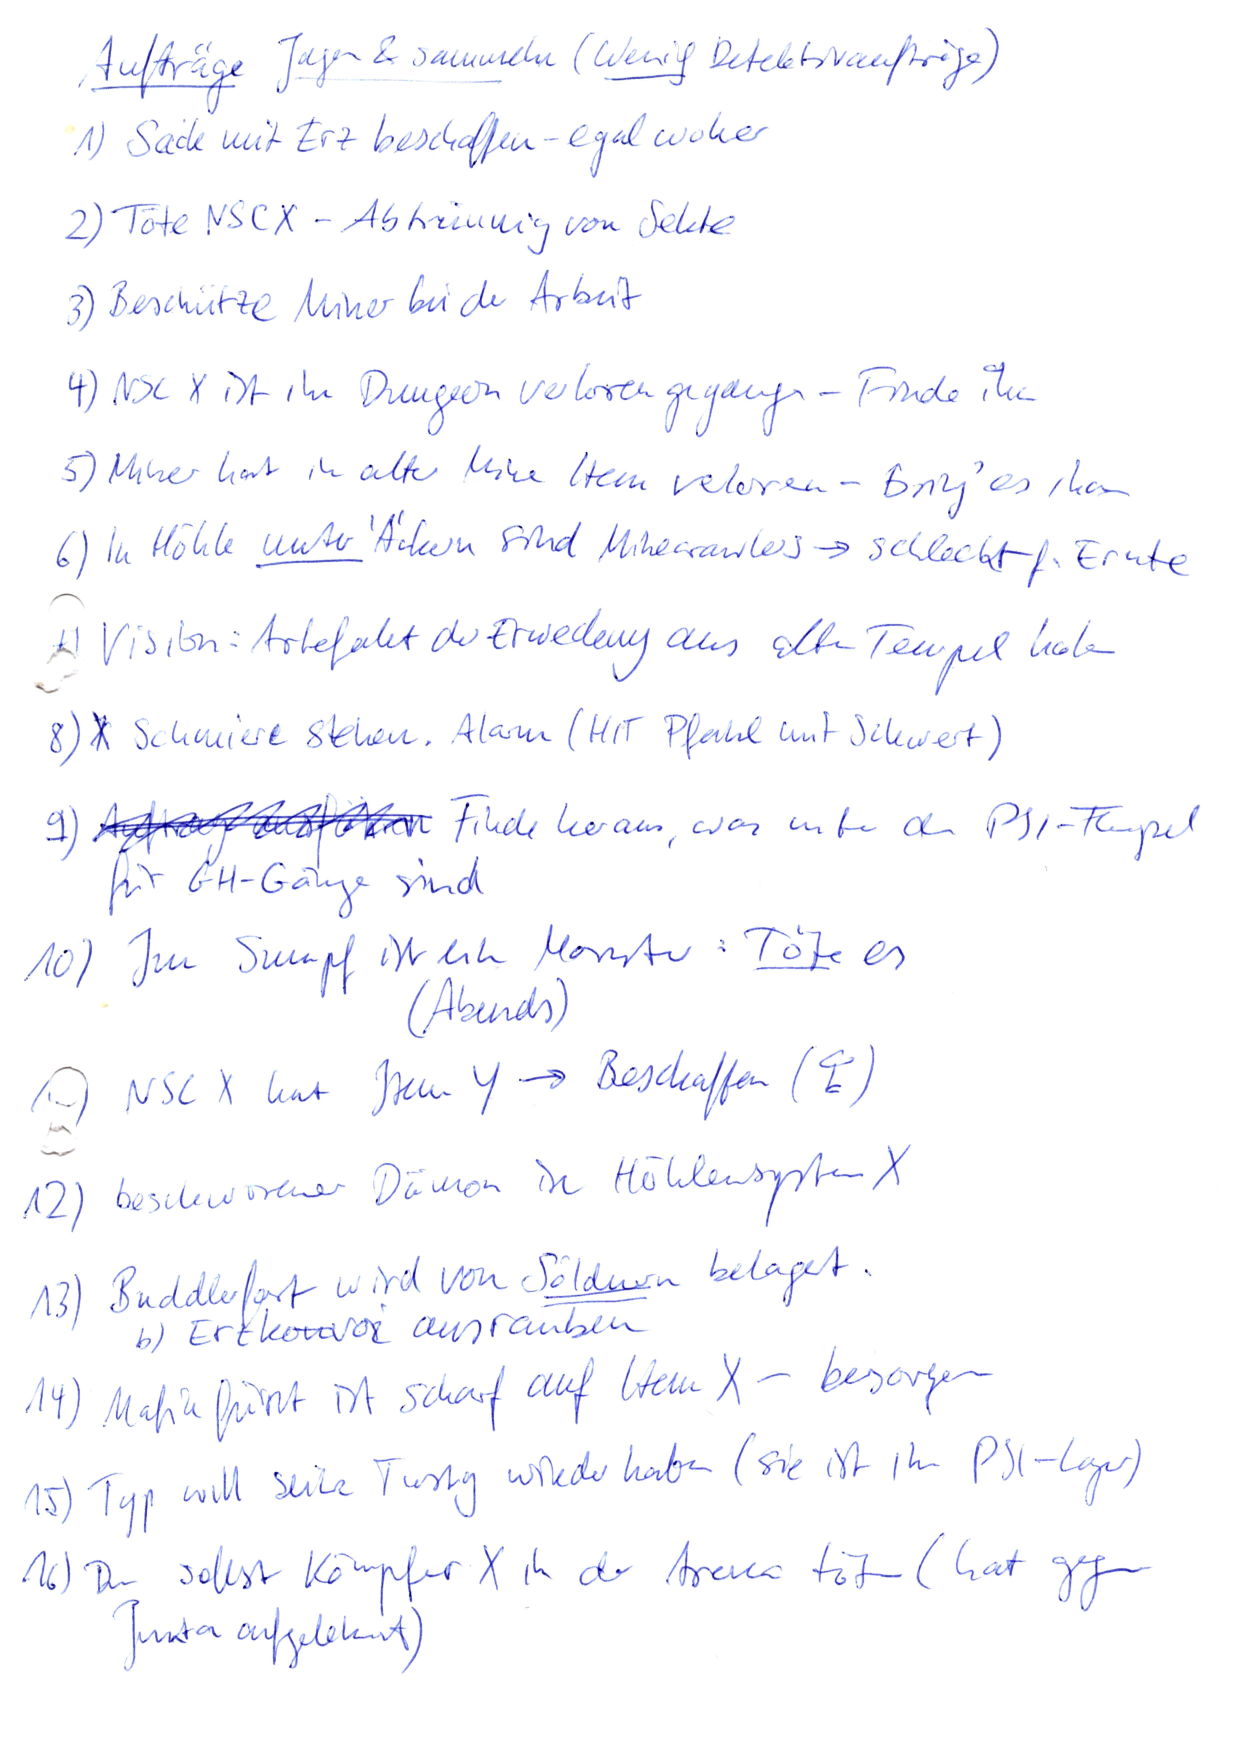
\includegraphics[scale=0.5]{orpheus_auftraege.pdf}}
   \caption{Ausschnitt aus \enquote{\uline{Aufträge}}}
   \label{fig:orpheus_auftraege}
\end{figure}


%%%%%%%%%%%%%%%%%%%%%%%%
% ORPHEUS – SPIELWELT %
%%%%%%%%%%%%%%%%%%%%%%%
\clearpage
\section{Spielwelt}\label{sec:orpheus_welt}


%%%%%%%%%%%%%%%%%%%%%%%%
% ORPHEUS – GESCHICHTE %
%%%%%%%%%%%%%%%%%%%%%%%%
\clearpage
\section{Geschichte}\label{sec:orpheus_geschichte}


%%%%%%%%%%%%%%%%%%%%%%%%%%%%%%%
% ORPHEUS – DISKONTINUITAETEN %
%%%%%%%%%%%%%%%%%%%%%%%%%%%%%%%
\clearpage
\section{(Dis-)Kontinuitäten}\label{sec:orpheus_diskontinuitaeten}


%%%%%%%%%%%%%%%%
% BIBLIOGRAFIE %
%%%%%%%%%%%%%%%%
\clearpage
\addcontentsline{toc}{chapter}{Literaturverzeichnis}
\printbibliography


%%%%%%%%%%%%
% APPENDIX %
%%%%%%%%%%%%
\clearpage
\appendix


\end{document}
